\documentclass[12pt,a4paper]{article}

% Language setting
\usepackage[british]{babel}

% Set page size and margins
\usepackage[a4paper,top=2cm,bottom=2cm,left=2.5cm,right=2.5cm,marginparwidth=1.75cm]{geometry}

%----------- APA style references & citations (starting) ---
% Useful packages
%\usepackage[natbibapa]{apacite} % APA-style citations.

\usepackage[style=apa, backend=biber]{biblatex} % APA 7th edition style citations using biblatex
\addbibresource{references.bib} % Your .bib file

% Formatting DOI in APA-7 style
%\renewcommand{\doiprefix}{https://doi.org/}

% Add additional APA 7th edition requirements
\DeclareLanguageMapping{british}{british-apa} % Set language mapping
\DeclareFieldFormat[article]{volume}{\apanum{#1}} % Format volume number

% Modify 'and' to '&' in the bibliography
\renewcommand*{\finalnamedelim}{%
  \ifnumgreater{\value{liststop}}{2}{\finalandcomma}{}%
  \addspace\&\space}
  
%----------- APA style references & citations (ending) ---


\usepackage{amsmath}
\usepackage{graphicx}
\usepackage[colorlinks=true, allcolors=blue]{hyperref}
\usepackage{hyperref}
%\usepackage{orcidlink}
\usepackage[title]{appendix}
\usepackage{mathrsfs}
\usepackage{amsfonts}
\usepackage{booktabs}       % For \toprule, \midrule, \botrule
\usepackage{threeparttable} % For table footnotes
\usepackage{algorithm}
\usepackage{algorithmicx}
\usepackage{algpseudocode}
\usepackage{listings}
\usepackage{enumitem}
\usepackage{chngcntr}
\usepackage{booktabs}
\usepackage{lipsum}
\usepackage{subcaption}
\usepackage{authblk}
\usepackage[T1]{fontenc}    % Font encoding
\usepackage{csquotes}       % Include csquotes
\usepackage{diagbox}
\usepackage{comment}
\usepackage{url}

%\usepackage[justification=raggedright, singlelinecheck=false]{caption}
\usepackage{helvet}  % Load Helvetica (Arial-like)
\usepackage{lmodern}  % Ensures default LaTeX font is available

% label format: capital, centering, and parens
\renewcommand{\thesubfigure}{\Alph{subfigure}}

% Customize line spacing
\usepackage{setspace}
\onehalfspacing % 1.5 line spacing

% Redefine section and subsection numbering format
\usepackage{titlesec}
\titleformat{\section} % Redefine section numbering format
  {\normalfont\Large\bfseries}{\thesection.}{1em}{}
  
% Customize line numbering format to right-align line numbers
%\usepackage{lineno} % Add the lineno package
%\renewcommand\linenumberfont{\normalfont\scriptsize\sffamily\color{blue}}
%\rightlinenumbers % Right-align line numbers

%\linenumbers % Enable line numbering

% Define a new command for the fourth-level title.
\newcommand{\subsubsubsection}[1]{%
  \vspace{\baselineskip}% Add some space
  \noindent\textbf{#1\\}\quad% Adjust formatting as needed
}
% Change the position of the table caption above the table
\usepackage{float}   % for customizing caption position
\usepackage{caption}
\captionsetup[table]{position=top} % caption position for tables
\captionsetup[table]{labelfont=bf} % caption label
\captionsetup[figure]{labelfont=bf} % caption label

% Define the unnumbered list
\makeatletter
\newenvironment{unlist}{%
  \begin{list}{}{%
    \setlength{\labelwidth}{0pt}%
    \setlength{\labelsep}{0pt}%
    \setlength{\leftmargin}{2em}%
    \setlength{\itemindent}{-2em}%
    \setlength{\topsep}{\medskipamount}%
    \setlength{\itemsep}{3pt}%
  }%
}{%
  \end{list}%
}
\makeatother

% Suppress the warning about \@parboxrestore
\pdfsuppresswarningpagegroup=1

\date{}  % Remove date


\begin{document}


%----------


\begin{center}
{\Huge A Digital Twin Framework for Risk Assessment in Construction Scheduling: Integrating Monte Carlo and Bayesian Network Approaches}
\\[4ex]

\noindent
{\large Nilson Jorge Leão Junior} \\
{\small
Engineering College, Federal University of Catalão (UFCAT), Catalão, Goiás 75701-180, Brazil \\
nilsonjorgejunior@gmail.com \\
\url{https://orcid.org/0000-0000-0000-0000}
} \\[1.2em]

{\large Wanderlei Malaquias Pereira Junior \small(Corresponding Author)} \\
{\small
Engineering College, Federal University of Catalão (UFCAT), Catalão, Goiás 75701-180, Brazil \\
wanderlei\_junior@ufcat.edu.br \\
\url{https://orcid.org/0000-0000-0000-0000}
} \\[1.2em]

{\large Henrique de Oliveira Caetano} \\
{\small
São Carlos School of Engineering (EESC), University of São Paulo (USP), São Carlos, São Paulo 13566-590, Brazil \\
henrique.caetano@usp.br \\
\url{https://orcid.org/0000-0000-0000-0000}
} \\[1.2em]

{\large Marcos Luiz Henrique} \\
{\small
NICEN - Interdisciplinary Center for Exact and Natural Sciences, Caruaru, Pernambuco 55014-900, Brazil \\
marcos.luiz@nicen.br \\
\url{https://orcid.org/0000-0000-0000-0000}
} \\[1.2em]

{\large Marcos Napoleão Rabelo} \\
{\small
Engineering College, Federal University of Catalão (UFCAT), Catalão, Goiás 75701-180, Brazil \\
marcos.rabelo@ufcat.edu.br \\
\url{https://orcid.org/0000-0000-0000-0000}
} \\[1.2em]

{\large Toni Esteves} \\
{\small
Department of Computer Science, Federal University of Minas Gerais (UFMG), Belo Horizonte, Minas Gerais 31270-901, Brazil \\
toni.esteves@dcc.ufmg.br \\
\url{https://orcid.org/0000-0000-0000-0000}
} \\[1.2em]

{\large Hebert Kimura} \\
{\small
Faculty of Economics, Administration, Accounting and Actuarial Science (FACE), University of Brasília (UnB), Brasília, Distrito Federal 70910-900, Brazil \\
hebert.kimura@unb.br \\
\url{https://orcid.org/0000-0000-0000-0000}
} \\[1.2em]

{\large Carlos Dias Maciel} \\
{\small
Engineering College, São Paulo State University (UNESP), Guaratinguetá, São Paulo 12516-410, Brazil \\
carlos.maciel@unesp.br \\
\url{https://orcid.org/0000-0000-0000-0000}
}
\end{center}

\begin{abstract}
Abstracts must be able to stand alone and so cannot contain citations to the paper’s references, equations, etc. An abstract must consist of a single paragraph and be concise. Because of online formatting, abstracts must appear as plain as possible. Three to six keywords must be included. Each keyword should not exceed three words. %\lipsum[1]
\end{abstract}

\textbf{Keywords}: keyword1, keyword2, keyword3, keyword4, keyword5, keyword6.  

%-------------------------------------------
% Paper Body
%-------------------------------------------
%--- Section ---%
\section*{Nomenclature}

\begin{tabbing}
$T$\qquad \= Temperature (K)\\
$u_i$ \> Velocity in the x-direction (m/s)\\
$\tau_{ij}$ \> Shear stress (N/m2)\\
$\omega$ \> Specific turbulent dissipation rate (1/s)\\
$Y_\omega$ \> Dissipation of $\omega$
\end{tabbing}

\section{Introduction}\label{sec:intro}The construction sector is among the world’s largest industries, with annual expenditures of roughly USD 10 trillion on construction goods and services, representing approximately 13\% of global Gross Domestic Product (GDP) in 2023, and is expected to grow to USD 33 trillion by 2040 \citep{Singh2026}. 

Due to their dynamic and demanding context, engineering projects operate under increasingly compressed timelines, complex supply chains, and stringent performance requirements. Within this operational environment, the construction schedule becomes a mission-critical asset, serving as the primary mechanism for resource orchestration, activity coordination, and alignment across multidisciplinary stakeholders.

Scheduling problems in construction projects lead to negative outcomes, including delays and rework \citep{Kline2025}. Despite its critical importance in construction projects, scheduling is often underemphasized in formal engineering education. Consequently, construction and project management professionals tend to acquire skills in developing workable schedules primarily through on-the-job experience \citep{Vahidi2025}.

In this paper, we develop a digital twin framework to assess risk in construction scheduling. We explore the traditional PERT (Program Evaluation and Review Technique) and CPM (Critical Path Method) methods within a probabilistic framework to estimate scheduling risk metrics. Uncertainty and dependence of the duration of each project's activities are taken into account using Monte Carlo simulation and Bayesian Networks. 

The paper is structured as follows. In the next section, we present the key tools and techniques for assessing scheduling risks. We then briefly discuss the digital twin framework and contextualize the proposed model. We describe the architecture of the proposed framework and discuss the results obtained from its application to assess scheduling risks, using a toy problem in civil engineering. We present characteristics of the implemented system, including details of the simulation mechanism and risk analysis. Finally, we make concluding remarks, highlighting the applications and limitations of the study.


\section{Theoretical Background}\label{sec:theory}In this paper, we employ traditional PERT and CPM concepts to develop a framework for assessing engineering project schedules. However, in this study, we address uncertainty by incorporating possible scenarios, using metrics based on financial risk management: Value-at-Risk and Expected Shortfall, allowing a more realistic analysis of scheduling risk. We analyse uncertainty using Monte Carlo simulation and Bayesian Networks, from a digital twin perspective. 

The following sections present the theoretical background underlying these methods and their applications within the proposed framework. 

\subsection{PERT/CPM and Graphs}

This paper explores PERT and CPM to analyse the risk of the engineering project schedule. The early and seminal works of PERT \citep{Malcolm1959, Clark1962, Elmaghraby1967} and CPM \citep{Kelley1961, Fulkerson1961} provide practical motivation and mathematical underpinnings for these techniques, which are widely used in engineering and construction planning. 

In the following sections, we briefly present the theoretical background underlying these methods and their application within our proposed framework.

 
\subsubsection{Events and Activities}
Engineering projects can be decomposed into a structured set of activities, each representing a well-defined component of the overall work. In a probabilistic scheduling environment, the duration of each activity may be characterised by a probability density function that captures inherent uncertainties. Logical constraints between activities, expressed as precedence relationships, define how these elements are connected within the project network \cite{bagshaw2011, moder2020}. 


In the PERT/CPM formulation, there are two main approaches to represent the precedence of activities in a project 
 \citep{jafari2019, singh2018}: 

\begin{itemize}
    \item Activity on Arc (AOA): Activities are represented by arcs and events by nodes. Each arc shows the duration of the activity. Dummy activities may be used to preserve correct precedence relationships.
    
    \item Activity on Node (AON): Activities are represented by nodes and precedence relationships by arrows connecting them. This approach is generally easier to construct and avoids the need for dummy activities.
\end{itemize}

 
\label{subsec:graph_approach}
%\subsubsection{Graph Approach}

%A PERT/CPM network can be represented as a directed, connected, and acyclic graph \( G(V, A) \), where \( V = \{ v_1, v_2, \ldots, v_n \} \) is the set of nodes (events) and \( A = \{ a_1, a_2, \ldots, a_m \} \) is the set of arcs. %(activities).\textcolor{red}{XXX incluir referencias}
%Events are indexed such that an event \( v_i \) precedes an event \( v_j \), with \( i < j \), whenever an activity exists from \( v_i \) to \( v_j \). 

%The initial event \( v_1 \) and the final event \( v_n \) represent the start and completion of the project.
%In the probabilistic formulation, the duration \( t_k \) of each activity \( a_k \in A \) is modeled as a non-negative random variable, capturing the uncertainty inherent in engineering and construction operations.
%Let \(R = \{ r_1, r_2, \ldots, r_{|R|} \},\) be the set of all simple paths connecting events \( v_1 \) and \( v_n \), where \( |R| \) denotes the cardinality of this set.

%The duration \( T_j \) of a path \( r_j \in R \) is defined as:

%\begin{equation}
%T_j = \sum_{a_k \in r_j} t_k .
%\label{eq:path_duration}
%\end{equation}
%%%%%%%%%%% Marcos Henrique%%%%%
\subsubsection{Graph Approach}
\begin{figure}[h]
    \centering
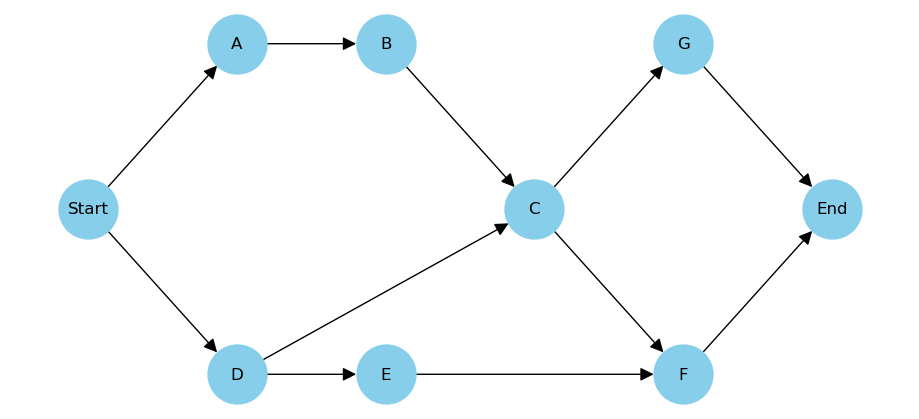
\includegraphics[width=0.6\linewidth]{images/fig_grafo_direcionado.png}
    \caption{Graph of the project plan.}
    \label{fig:031024}
\end{figure}

A PERT/CPM network is represented as a directed, connected, and acyclic graph   
\( G = (V, A) \), where 
\( V = \{ v_1, v_2, \ldots, v_n \} \) denotes the set of nodes, each corresponding to an activity, and 
\( A \subseteq V \times V \) denotes the set of directed arcs representing precedence relations between activities \citep{bagshaw2021pert}. An arc \( (v_i, v_j) \in A \) represents a precedence relation in which activity \( v_j \) starts after the completion of activity \( v_i \), with \( i < j \).

The graph is structured so that \( v_1 \) and \( v_n \) represent the start and completion of the project, respectively, corresponding to dummy activities of zero duration, thereby defining complete execution paths.

In the probabilistic formulation, the duration \( t_i \) associated with each activity node \( v_i \in V \) is modelled as a non-negative random variable, capturing the uncertainty inherent in engineering and construction operations.

Let \( R = \{ r_1, r_2, \ldots, r_{|R|} \} \) denote the set of all simple paths that connect the initial activity \( v_1 \) and the terminal activity \( v_n \), where \( |R| \) denotes the cardinality of this set.

The duration \( T_j \) of a path \( r_j \in R \) is defined as the sum of the durations of the activities along the path:
\begin{equation}
T_j = \sum_{v_i \in r_j} t_i .
\label{eq:path_duration}
\end{equation}

%%%%%%%%%%%%%%%%%%%%%%%
\subsubsection{Critical Path}

The duration of a schedule is determined by the temporal constraints of the network activities. That if there is a path from the origin event ($v_1$) to the terminus event ($v_n$) whose length equals the duration of the schedule, this path is designated as a \textit{critical path} \citep{Kelley1961}.

Mathematically, considering the set of all path durations computed in Eq. (1), the project duration ($T_{project}$) corresponds to the maximum value among all possible paths $r_j \in R$. Thus, the critical path determines the minimum time required to complete the project:

\begin{equation}
T_{project} = \max_{r_j \in R} \{ T_j \} \quad (2)
\end{equation}

Activities located on this path are termed \textit{critical activities}. These activities are limiting in that any delay in one of them will cause a comparable delay in project completion \citep{Kelley1961}. In terms of float analysis, critical activities are characterised by having a total float equal to zero, meaning the maximum time available for the activity equals its duration.

Since this study considers the durations of activities $t_k$ as random variables, the inequality $T_{project} \ge T_j$ holds for all $j$, but the specific path that satisfies the condition of maximum duration can vary between different simulation scenarios.

\label{sub:var}
\subsection{Risk management metrics}
We briefly discuss two very common risk management metrics, Value--at--Risk and Expected Shortfall), that are extensively used in the finance industry. These metrics are used by banks and regulators to quantitatively assess market, credit, and operational risk, and their concepts can be adapted for the construction industry. 


\subsubsection{Value--at--Risk}

Introduced by J.P. Morgan and Reuters in the 1990s, Value-at-Risk (VaR) is a risk metric now widely used in finance and adapted to other industries. The $VaR$ is based on quantiles of the profit-and-loss distribution of a financial portfolio and measures the amount a portfolio or asset might lose over a specified time horizon with a given confidence level \citep{Riskmetrics}.

Although originally applied to assess potential monetary loss, the concept $VaR$ can also be utilised in other non-financial applications. In our study, we use the quantile interpretation of $VaR$ based on confidence level to analyse the risk of scheduling.   

%Com a amostragem probabilistica de dias X que uma dada atividade pode durar é possível determinar com um nível de confiança $\alpha$ que aquela atividade dure até ${{VaR}_{\alpha}}$ dias.
 
Within this a probabilistic approach, if $X$ is a random variable that describes the duration (e.g. number of days) of an activity of the project, and $1-\alpha$ is the confidence level (e.g. $1-\alpha=95\%$, where $\alpha=5\%$ is the tail probability), then the $VaR$ is the $\alpha$--quantile of the loss distribution, at a confidence level $1-\alpha$, and is defined as:
 
\begin{equation}
    P(X > \text{VaR}_{\alpha})= \alpha
\end{equation}

In the scheduling context, $VaR$ measures the tail probability of an activity's duration (i.e., the maximum duration) at a given confidence level. 

\subsubsection{Expected Shortfall}
The Expected Shortfall ($ES$), also called Conditional Value-at-Risk ($CVaR$), is another widely used risk metric in finance that indicates the expected loss conditional on exceeding the $VaR$ \citep{Artzner1999, Acerbi2002}. From a scheduling perspective, $ES$ identifies the expected value of the duration of an activity conditional on exceeding $VaR$. 

\begin{equation}
ES_{\alpha}(X) = \mathbb{E}\!\left[\, X \mid X \ge \text{VaR}_{\alpha}(X) \,\right]
\end{equation}

Therefore, $VaR_{\alpha}$ would express the maximum duration of an activity, with a predefined confidence level $1-\alpha$, while $ES_{\alpha}$ expresses the expected value of the duration of the activity, in the case it lasts longer than $VaR_{\alpha}$.

\subsection{Bayesian Network and Evidence Propagation}

To formally model the dependencies and uncertainties within [the system under study], we employ a \textbf{Probabilistic Graphical Model (PGM)}, specifically a Bayesian Network (BN). PGMs provide a robust formalism for representing complex stochastic systems by combining principles from graph theory and probability theory.

A Bayesian Network is formally defined by two components. The first is a qualitative structure, a Directed Acyclic Graph (DAG) $\mathcal{G} = (\mathbf{V}, \mathbf{E})$, in which nodes $\mathbf{V}$ correspond to random variables and directed edges $\mathbf{E}$ represent conditional dependencies \citep{caetano2024resilience}. 

The structure of this DAG is fundamental because it encodes a set of conditional-independence assumptions over the domain. These assumptions, in turn, enable an efficient decomposition of the joint probability distribution over the set of all variables $\mathbf{X} = \{X_1, \dots, X_n\}$. Instead of relying on the full chain rule of probability, the distribution factorises according to the graph structure:

\begin{equation}
P(X_1, \dots, X_n) = \prod_{i=1}^{n} P(X_i | \text{pa}(X_i))
\end{equation}

where $\text{pa}(X_i)$ is the set of parents for node $X_i$ in $\mathcal{G}$. The second component of a BN is a set of quantitative parameters, consisting of a Conditional Probability Table (CPT) for each node $X_i$. Each CPT quantifies the local distribution $P(X_i | \text{pa}(X_i))$, completing the probabilistic specification of the model. This factorisation is the core strength of BNs, drastically reducing the complexity of representation and inference.

\subsection{Probabilistic Inference and Evidence Propagation}
\label{subsec:evidence_propagation}

A primary application of Bayesian Networks is probabilistic inference, which involves updating the beliefs about certain variables upon observing new information, known as \textbf{evidence}. This process, often termed \textbf{evidence propagation} or belief updating, allows the model to perform diagnostic and predictive reasoning \citep{pearl1988probabilistic}.

Formally, let the set of all variables in the network be $\mathbf{X} = \{X_1, \dots, X_n\}$. Evidence, denoted as $\mathbf{e}$, is an instantiation of a subset of evidence variables $\mathbf{E} \subseteq \mathbf{X}$ to specific states. The objective of inference is to compute the posterior probability distribution of a set of query variables $\mathbf{Q} \subseteq \mathbf{X} \setminus \mathbf{E}$, given the evidence $\mathbf{e}$. That is, our goal is to compute $P(\mathbf{Q} | \mathbf{E} = \mathbf{e})$.

The foundation for this belief update is Bayes' theorem. For a single query variable $X_i$ and a set of evidence $\mathbf{e}$, the posterior probability is calculated as follows \citep{pearl2022external}:
%
\begin{equation}
\label{eq:evidence_prob_update}
\underbrace{P(X_i | \mathbf{e})}_{\text{Posterior}} = \frac{\overbrace{P(\mathbf{e} | X_i)}^{\text{Likelihood}} \cdot \overbrace{P(X_i)}^{\text{Prior}}}{\underbrace{P(\mathbf{e})}_{\text{Evidence}}}
\end{equation}
%
In Equation \ref{eq:evidence_prob_update}, each term has a distinct role:
\begin{itemize}
    \item $P(X_i)$ is the \textbf{prior probability} of $X_i$, representing the belief about the variable before any evidence is observed. It can be computed from the joint distribution defined by the BN.
    \item $P(\mathbf{e} | X_i)$ is the \textbf{likelihood}, which quantifies the probability of observing the evidence $\mathbf{e}$ for each possible state of the query variable $X_i$.
    \item $P(X_i | \mathbf{e})$ is the \textbf{posterior probability}, representing the updated belief about $X_i$ after considering the evidence.
    \item $P(\mathbf{e})$ is the \textbf{marginal likelihood} of the evidence, which acts as a normalisation constant to ensure that the posterior probabilities sum to one.
\end{itemize}

The marginal likelihood $P(\mathbf{e})$ is computed by summing the joint probabilities over all possible states of the query variable $X_i$, an application of the law of total probability. Assuming $X_i$ can take on states $\{x_{i1}, \dots, x_{ik}\}$, it is given by:
%
\begin{equation}
\label{eq:sum_denominador}
P(\mathbf{e}) = \sum_{j=1}^{k} P(\mathbf{e} | X_i = x_{ij}) P(X_i = x_{ij})
\end{equation}
%
This framework allows for the computation of probabilities that are often difficult to assess directly, such as $P(X_i | \mathbf{e})$, by leveraging more intuitive or empirically derivable quantities like the prior and the likelihood \cite{caetano2024resilience}.
\section{Digital Twin Framework}\label{sec:dtwin}A Digital Twin (DT) is formally defined as a digital representation of a physical item or assembly, using integrated simulations and service data. Designed to predict current and future conditions in both design and operational environments to improve decision-making, the digital representation integrates information from multiple sources throughout the product life cycle and is continuously updated \citep{fuller2020, jiang2021}.

The fundamental characteristic of DT is the level of data integration, classifying the models into three levels: (a) Digital model: it is a digital version of a physical object where there is no automatic switching between the physical model and the digital model; (b) Digital shadow: it has a unidirectional data flow, and therefore, changes to a physical object automatically change the digital object, but the reverse is not true; and (c) Digital Twin: it is defined by the complete integration of data flow in both directions \citep{iranshahi2025digital}.

Table \ref{tab:digital_capabilities} presents a consolidated overview of the capabilities and progression levels associated with Digital Models, Digital Shadows, and Digital Twins. As illustrated in Figure \ref{fig:dt_levels}, these three paradigms differ fundamentally in terms of data integration, automation maturity, and real-time interaction between physical and digital assets.

\begin{table}[htbp!]
\centering
\caption{Comparing the capabilities of Digital Twins, Digital Shadows, and Digital Models in performing different functions \citep{iranshahi2025digital}.}
\label{tab:digital_capabilities}
\begin{tabular}{p{7cm}ccc}
\toprule
\textbf{Functions} & \textbf{Digital Model} & \textbf{Digital Shadow} & \textbf{Digital Twin} \\
\midrule
Automatic data flow; from physical object to digital model. & $\times$ & $\checkmark$ & $\checkmark$ \\
Automatic data flow; from digital model to physical object. & $\times$ & $\times$ & $\checkmark$ \\
Predictive analysis; Testing scenarios virtually before applying them physically. & $\checkmark$ & $\checkmark$ & $\checkmark$ \\
Real-time monitoring of its real-world counterpart. & $\times$ & $\checkmark$ & $\checkmark$ \\
Decision-making; Real-time data analysis and predictive evaluation. & $\checkmark$ & $\checkmark$ & $\checkmark$ \\
Control; Real-time interaction and optimization of the physical system. & $\times$ & $\times$ & $\checkmark$ \\
\bottomrule
\end{tabular}
\end{table}


\begin{figure}[htbp!]
\centering
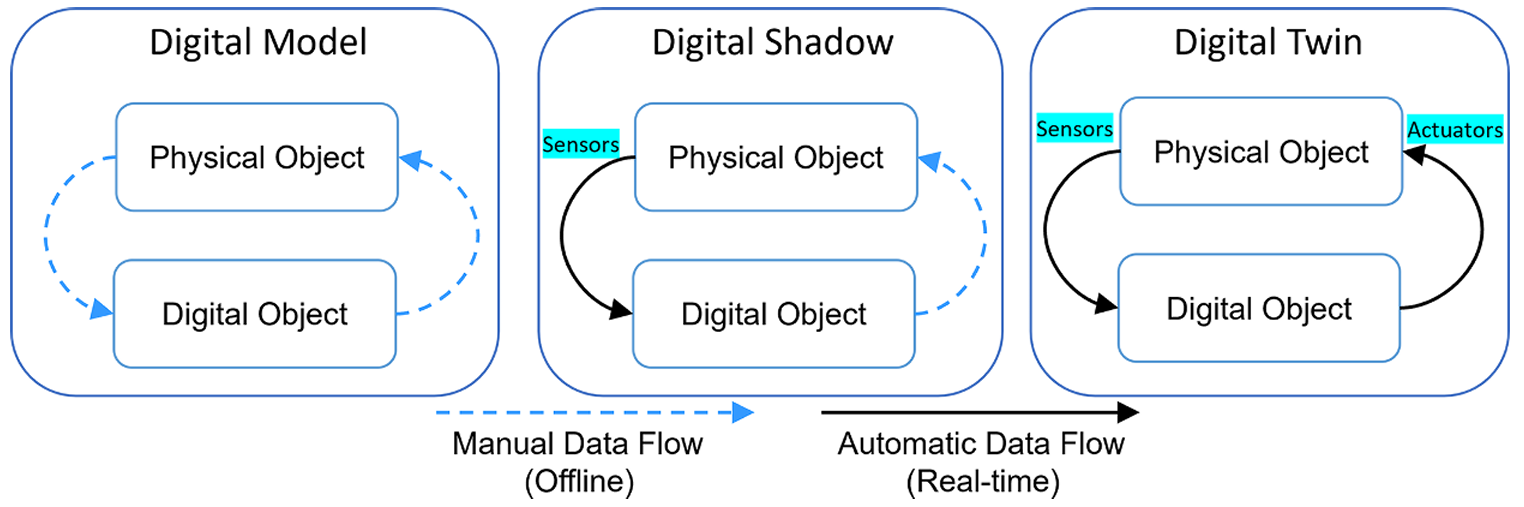
\includegraphics[width=0.85\textwidth]{z_fig_dt_level.png}
\caption{Conceptual differentiation among Digital Model, Digital Shadow, and Digital Twin based on data-flow direction and automation level \parencite{iranshahi2025digital}.}
\label{fig:dt_levels}
\end{figure}



\section{Implementation}\label{sec:impl}Following the taxonomy of \cite{kritzinger2018digital}, the proposed framework operates as a digital shadow rather than a fully bidirectional digital twin. Information flows from the physical project to the probabilistic digital representation through structured data uploads compiled by site engineers, while decisions derived from the model outputs remain mediated by human agents. This positioning reflects the operational reality of construction projects, where automated actuation on the physical system is precluded by contractual, regulatory, and human judgment constraints.

The framework is implemented in Python and exposed through a client and server architecture. A Streamlit based web interface \citep{streamlit} handles data ingestion and visualization, while the inference engine runs on the server side. Monte Carlo sampling of activity durations relies on the \texttt{Scipy}, which natively supports the triangular distributions adopted in this work, and Bayesian inference is performed with the library \texttt{pgmpy}. Activity durations are sampled with $N = 10,000$ realizations, a value consistent with the Monte Carlo sample sizes.% commonly adopted in stochastic CPM analysis [citar 1 ou 2 trabalhos]. 

The Bayesian network is constructed directly from the CPM precedence graph: each activity is mapped to a node, arcs follow the precedence relations, and conditional probability tables are estimated from the empirical relative frequencies of the sampled durations after discretization. The discretization resolution is a user defined parameter; integer days are adopted as the default because they match the operational granularity at which construction schedules are managed and reported, ensuring that each discrete state in the Bayesian network corresponds to an observation directly realizable in the field. 

The framework takes as input a simple activity table containing, for each activity, its identifier, predecessors, and the minimum, mode, and maximum duration values that parameterize the triangular distribution. A public web deployment of the tool is available at \url{https://civilprobabilisticplanning.streamlit.app}, where readers can reproduce the analyses presented in Section 5 and apply the framework to their own planning scenarios.

The digital twin assessment pipeline is divided into 3 categories or activities: (\textit{a}) uploading the desired scenario, (\textit{b}) choosing the adopted risk level, and (\textit{c}) applying the evidence concept and its propagation in the complex network. Each of these items is detailed to provide an overview of how the digital twin supports the desired planning analysis.

% \subsubsection{Dataset Upload and Critical Path Method Scenarios}

% The desired scenario dataset is transferred via a Streamlit file-upload component configured to accept only the \textit{xlsx} Excel format. Other formats are easy to implement. The file should contain a tab with the following columns properly filled in: (a) Code, (b) Task Name, (c) Predecessors, (d) Min., (e) Mode, (f) Max., and each row represents an activity in the plan. A scenario template is available in the application for download and editing to suit the user's plan.

% The ``\textit{Code}'' column contains the unique identifier for each activity. If the same identifier is present in more than one activity, the system will return an error as the application cannot perform the analyses correctly.

% The column ``\textit{Task Name}'' stores the name of the activity, which will be used as a visual identifier for the user during analysis. Therefore, we recommend that it also be represented by a unique value.

% The ``\textit{Predecessors}'' column indicates the code of the preceding activity. In the cases where there is more than one preceding activity, they must be separated by a comma. For the first activity in the scenario, this column should be filled with ``-''. The system supports only one initial activity, and the user must account for this when entering scenarios.

% Before running the application, the user must initially determine the duration (in days) of each activity and fill in the ``Min.'' column with the estimated minimum duration, the ``Mode'' column with the most likely duration (mode), and the ``Max.'' column with the maximum duration the activity can have.

% After data input, the simulator performs a probabilistic time analysis of all planning activities and ultimately returns a sample of 10,000 scenarios from the set of activities, regardless of their size. The sample size can be changed. However, in the initial versions of the software, this value was standardised. For scenario analysis and generation, we use the \textit{parepy-toolbox} library, which supports triangular distributions; therefore, the minimum, mode, and maximum durations of each activity must be specified. Figure \ref{fig:hist_active_1} shows the histogram of the sample distribution of a given activity with minimum, mode, and maximum values equal to 2.0, 3.0 and 6.0, respectively.

% \begin{figure}
%     \centering
% 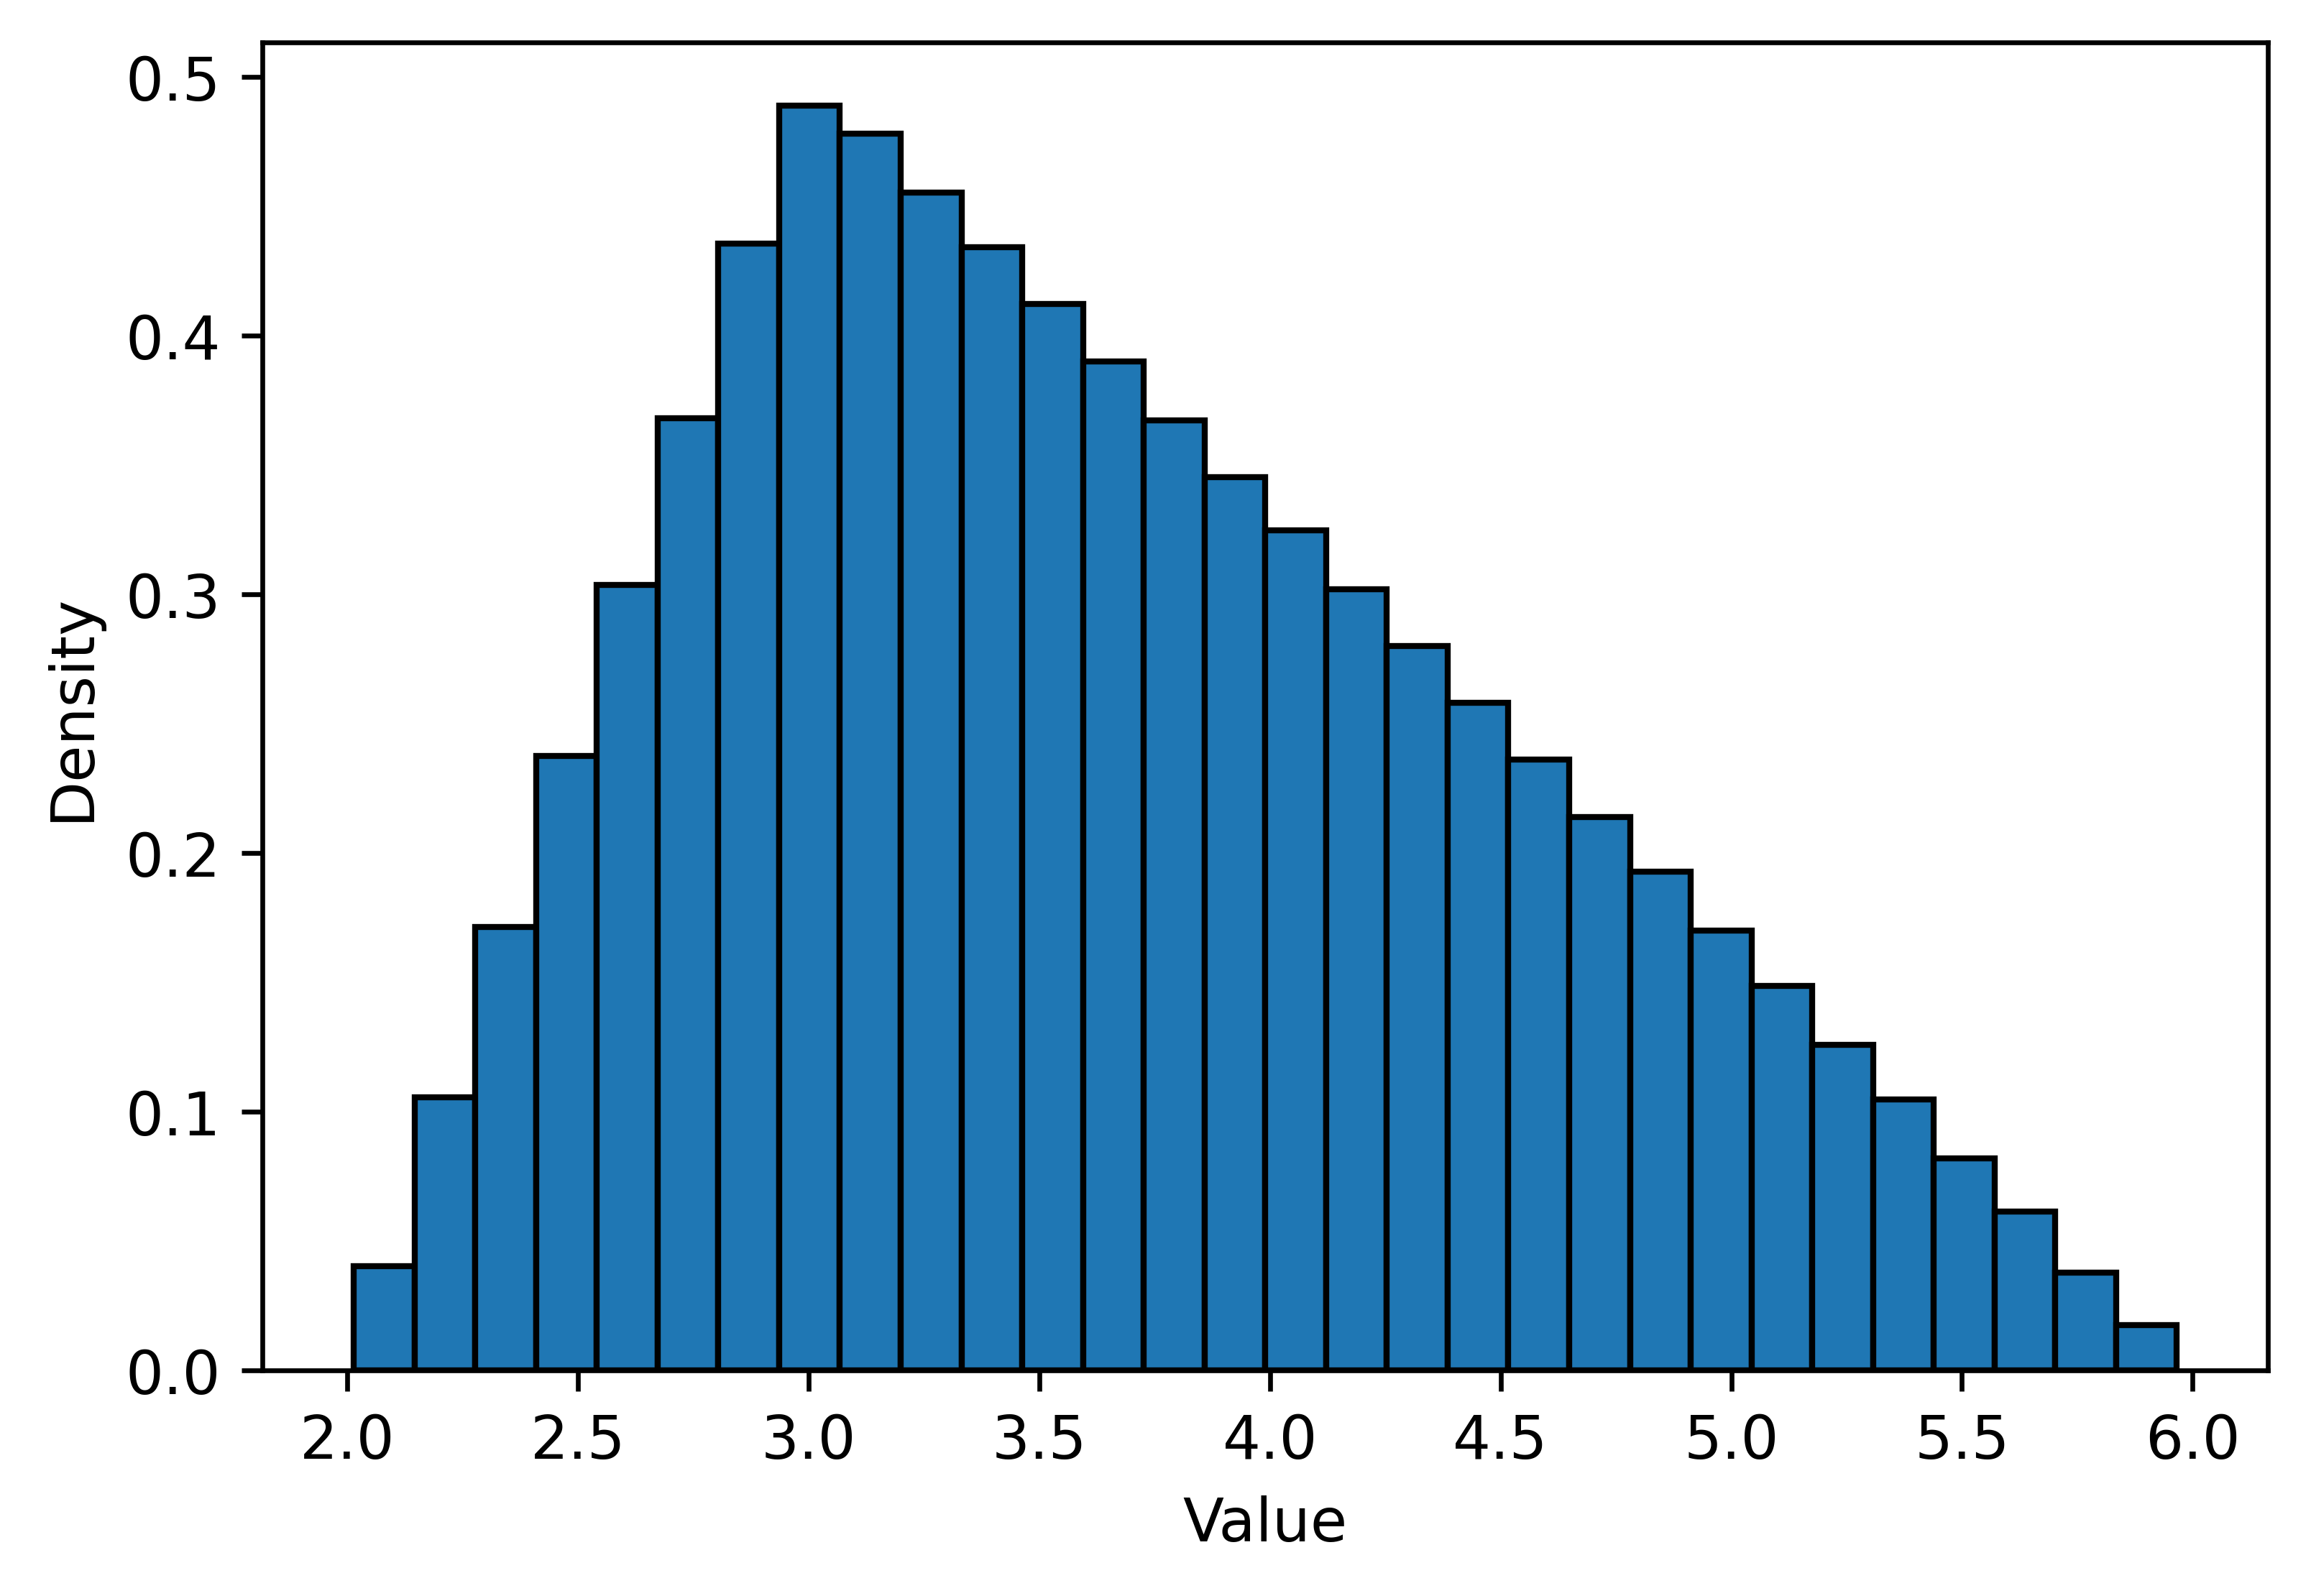
\includegraphics[width=0.6\linewidth]{images/fig_hist_active_1.png}
%     %\caption{Grafo do Plano  do projeto.}
%     \caption{Illustration of the histogram of an activity}
%     \label{fig:hist_active_1}
% \end{figure}


% \subsubsection{Risk analysis}

% Once the scenario database is built, the application provides functionality to perform risk analysis for the duration of the planning horizon; these concepts were explained in section \ref{sub:var}. To perform the risk analysis, the user must specify the desired confidence level, which must be between 0 and 1. The application will then display the VaR and CVaR for that planning horizon in days, based on the provided confidence level.

% \subsubsection{Belief propagation}

% The Bayesian Network is trained using Conditional Probability Tables (CPTs) derived from the scenario database. To compute the CPTs, data from all scenarios are first grouped by activity. The corresponding duration values are then rounded and discretized to identify a finite set of distinct states. Subsequently, the probability associated with each state is estimated from its empirical relative frequency, computed as the ratio between the number of occurrences of the state and the total number of observations in the dataset, as described in Algorithm~\ref{alg:discretization_integer_days}. Table~\ref{tab:cpt_example} presents an example of a resulting CPT obtained from the activity duration distribution illustrated in Figure~\ref{fig:hist_active_1}.

% \begin{algorithm}[H]
% \caption{Discretization by Integer Days}
% \label{alg:discretization_integer_days}
% \begin{algorithmic}[1]
% \REQUIRE $DF$ — matrix of continuous samples
% \ENSURE $\Theta$ — discretization parameters

% \STATE $DF^{*} \leftarrow \mathrm{round}(DF)$
% \STATE $\Theta \leftarrow \emptyset$

% \FOR{each activity $a$ in $DF^{*}$}
%     \STATE Compute relative frequencies of values in column $a$
%     \STATE $S_a \leftarrow$ sorted set of observed integer values
%     \STATE $P(s) \leftarrow$ empirical probability of each $s \in S_a$
%     \STATE Define value mapping $f_a(s) = s$
%     \STATE $\Theta[a] \leftarrow \{S_a, f_a, P(s)\}$
% \ENDFOR

% \RETURN $\Theta$
% \end{algorithmic}
% \end{algorithm}


% \begin{table}[h]
% \centering

% \caption{CPT of an activity}
% \begin{tabular}{cc}
% \toprule
% State & Probability \\
% \midrule
%  2 & 0.0625 \\
%  3 & 0.4167 \\
%  4 & 0.3333 \\
%  5 & 0.1667 \\
%  6 & 0.0208 \\
% \bottomrule
% \label{tab:cpt_example}
% \end{tabular}
% \end{table}

% Once the network is trained, the system allows the user to make inferences as the scheduled activities are completed. This enables updating the total project duration estimate based on observed performance. It is important to note that the values available for adding evidence are limited to the states defined in the CPT. Therefore, if an activity is completed with a duration outside the range (minimum and maximum) contained in the original dataset, the model will not allow the assignment of that specific value.

% After processing the inferences, the application generates an updated conditional probability distribution and presents the new project completion metrics. The system visually highlights the minimum and maximum duration scenarios, as well as the most likely value (mode of the distribution), allowing a clear view of the residual uncertainty in planning.

\subsection{Toy problem}
To illustrate the application of the digital model, a civil construction schedule is presented in Table \ref{tab:toyproblem}. This dataset represents a simplified planning scenario structured as a toy problem for methodological demonstration. The tasks follow well-defined precedence relationships, and their durations are specified using minimum, most likely, and maximum estimates, enabling controlled experimentation and comparative analysis within the proposed framework.

\begin{table}[htpb!]
    \centering
    \caption{Toy problem: civil construction schedule used to exemplify the application of the digital model, including task precedence relationships and minimum, most-likely, and maximum duration estimates.}
    \label{tab:toyproblem}
    \begin{tabular}{|l|l|l|l|l|l|}
    \hline
        \textbf{Code} & \textbf{Task Name} & \textbf{Predecessors} & \textbf{Min.} & \textbf{Mode} & \textbf{Max.} \\ \hline
        A & Activity 1 & -  & 0.5 & 1.0 & 2.0 \\ \hline
        B & Activity 2 & A  & 2.0 & 3.0 & 4.0 \\ \hline
        C & Activity 3 & A  & 0.5 & 1.0 & 1.5 \\ \hline
        D & Activity 4 & B  & 3.0 & 4.0 & 5.0 \\ \hline
        E & Activity 5 & C  & 2.0 & 3.0 & 6.0 \\ \hline
        F & Activity 6 & D,E & 1.8 & 2.0 & 4.0 \\ \hline
    \end{tabular}
\end{table}

\subsubsection{Scenarios}
%Mostra que a plataforma amostra cenários estatisticos do problema qie v quer analisar

%Com a inserção do dataset na plataforma, a mesma realiza a amostragem de 10000 cenários e disponibiliza da descrição estatística do novo dataset de amostras gerado conforme a figura \ref{fig:df_scenarios}.

Once the dataset is loaded onto the platform, it samples $10,000$ scenarios and provides a statistical description of the resulting sample. Figure \ref{fig:df_scenarios} shows the output of our system with the descriptive statistics for each task.



\begin{figure}
    \centering
    \fbox{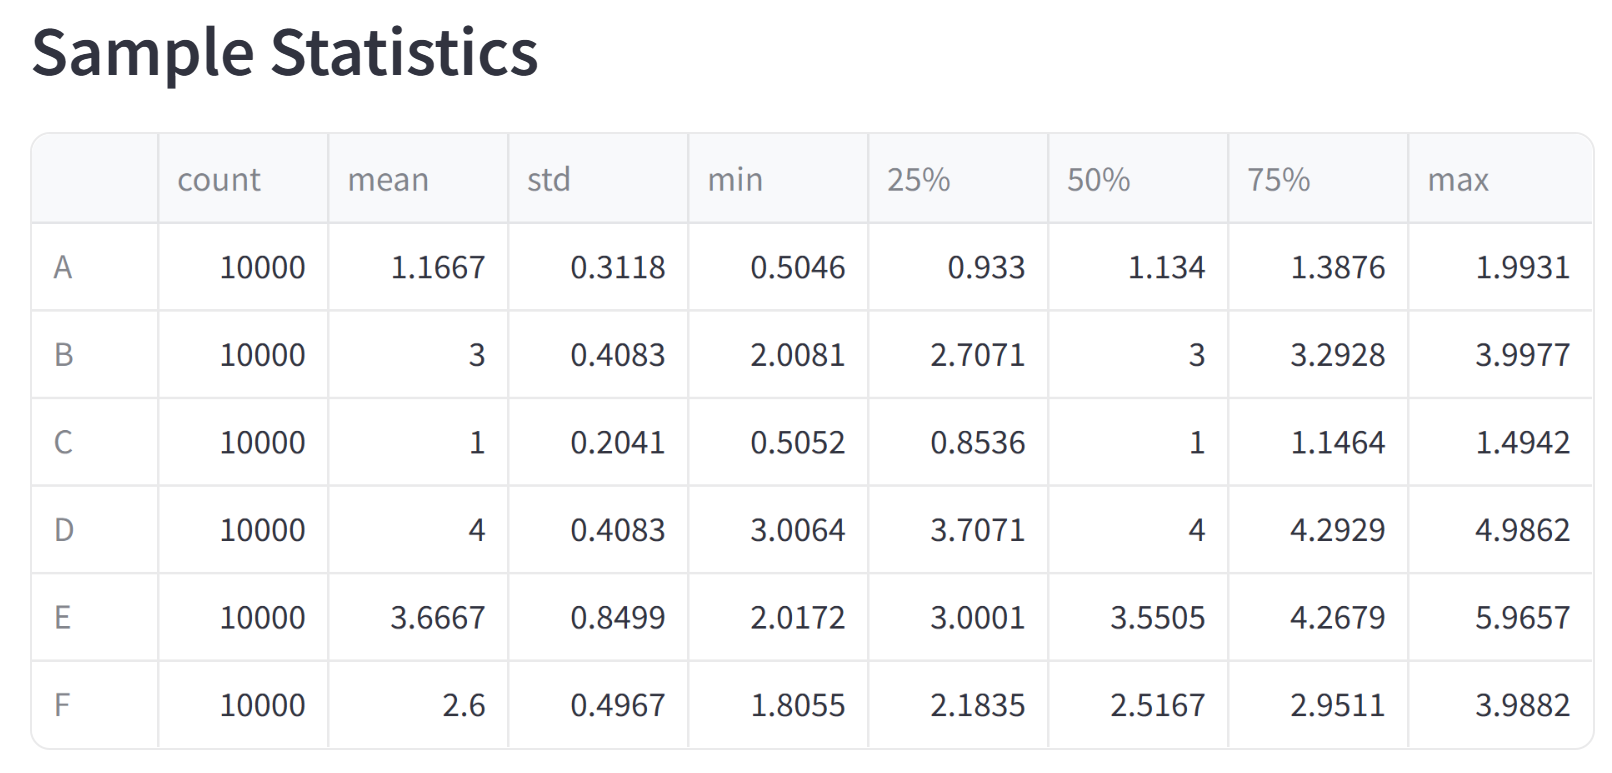
\includegraphics[width=1\linewidth]{images/sample_statistics.png}}
    \caption{System illustration: Description of the dataset containing all scenarios generated in the sampling.}
    \label{fig:df_scenarios}
\end{figure}

\subsubsection{Graph analysis and Critical Path}
%Mostra quais as capacidades do modelo em gerar cenários de caminho critico
%É possível fazer uma análise do grafo do dataset, definindo qual o ponto de início e o ponto de fim do caminho crítico, conforme a figura \ref{fig:graph_analysis}

We perform a graph analysis of the dataset, defining the starting point (activity 1) and ending point (activity 6) of the critical path, as shown in Figure \ref{fig:graph_analysis}.

\begin{figure}
    \centering
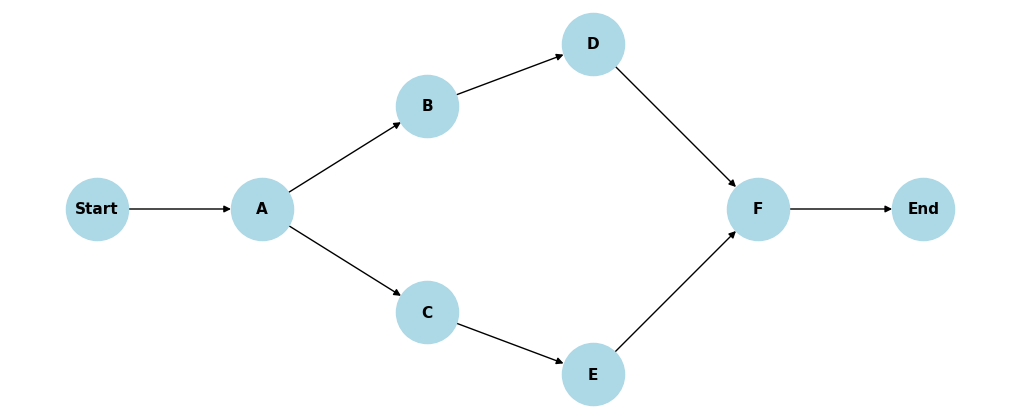
\includegraphics[width=0.6\linewidth]{images/fig2_grafo_direcionado.png}
    %\caption{Grafo do Plano  do projeto.}
    \caption{Graph of the project plan.}
    \label{fig2:031024}
\end{figure}

Figure \ref{fig:graph_analysis} illustrates the input interface of our system.

\begin{figure}
    \centering
    \fbox{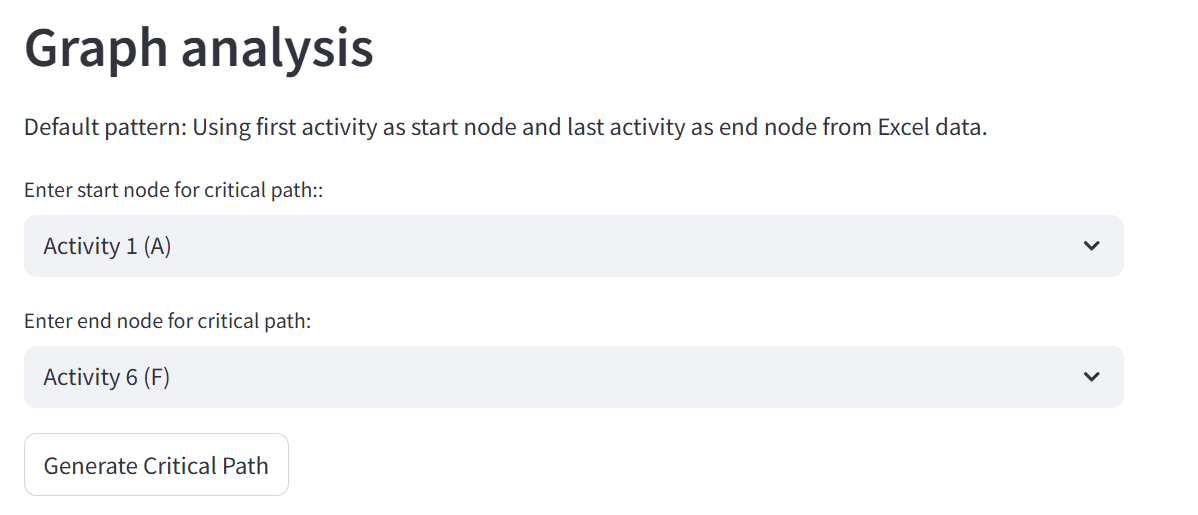
\includegraphics[width=1\linewidth]{images/define_path.png}}
    %\caption{Inputs para definir nó de início e nó de fim}
     \caption{System illustration: Inputs to define start node and end node.}
    \label{fig:graph_analysis}\end{figure}

%Para cada cenário gerado na amostragem, o sistema gera um grafo e o seu respectivo caminho crítico, ao fim disso é gerado um gráfico de densidade do tempo total daquele caminho crítico conforme a figura \ref{fig:makespan_scenarios}. Nesse gráfico é possivel observar que, para esse exemplo, grande parte dos cenários mostram que o planejamento irá durar 11 dias.

%HK. Acho quee a Figura 6 nao eh densidade. Eh um histograma (contendo a frequencia do tempo total). Funcao densidade de probabilidade eh mais usada para distribuicoes continuas. No caso, nao eh uma distribuicao de probabilidades, mas eh um histograma com a frequencia (observada)
For each scenario generated in the sampling, the system builds a graph and its respective critical path. The system also creates a histogram of the total time of that critical path, that could be a proxy of a probability distribution of the project makespan, as shown in figure \ref{fig:makespan_scenarios}.

The statistical descriptive analysis of the total project duration is summarized in Table \ref{tab:descriptive_stats}. The expected project makespan (mean) is 10.77 days, with a median of 10.75 days and a standard deviation of 0.82 days. The results range from a minimum of 8.10 days to a maximum of 13.90 days. Within this framework, we can identify that the most probable scenario (mode) is approximately 11 days.

\begin{table}[h]
\centering
\caption{Descriptive statistics of the project makespan (10,000 scenarios).}
\label{tab:descriptive_stats}
\begin{tabular}{l|r}
\hline
\textbf{Statistic} & \textbf{Value (Days)} \\ \hline
Sample Count & 10,000 \\
Mean & 10.77 \\
Standard Deviation & 0.82 \\
Minimum & 8.10 \\
First Quartile (25\%) & 10.20 \\
Median (50\%) & 10.75 \\
Third Quartile (75\%) & 11.32 \\
Maximum & 13.90 \\ \hline
\end{tabular}
\end{table}

%Within this framework, we can identify that the most probably scenario is that the planning will last 11 days. Other metrics can also be calculated. \textcolor{red}{Complementar For instance, the expected project makespan is XXXX (incluir o valor médio) and the standard deviation XXX (incluir o desvio-padrao). Talvez adcionar as principais estatisticas descritivas (minimo, media, mediana, maximo, desvio-padrao) da tarefa completa. Padronizar as tabelas e figuras (para nao ficar em formatos ou tamanhos ou fontes muito diferentes)}.

\begin{figure}
    \centering
    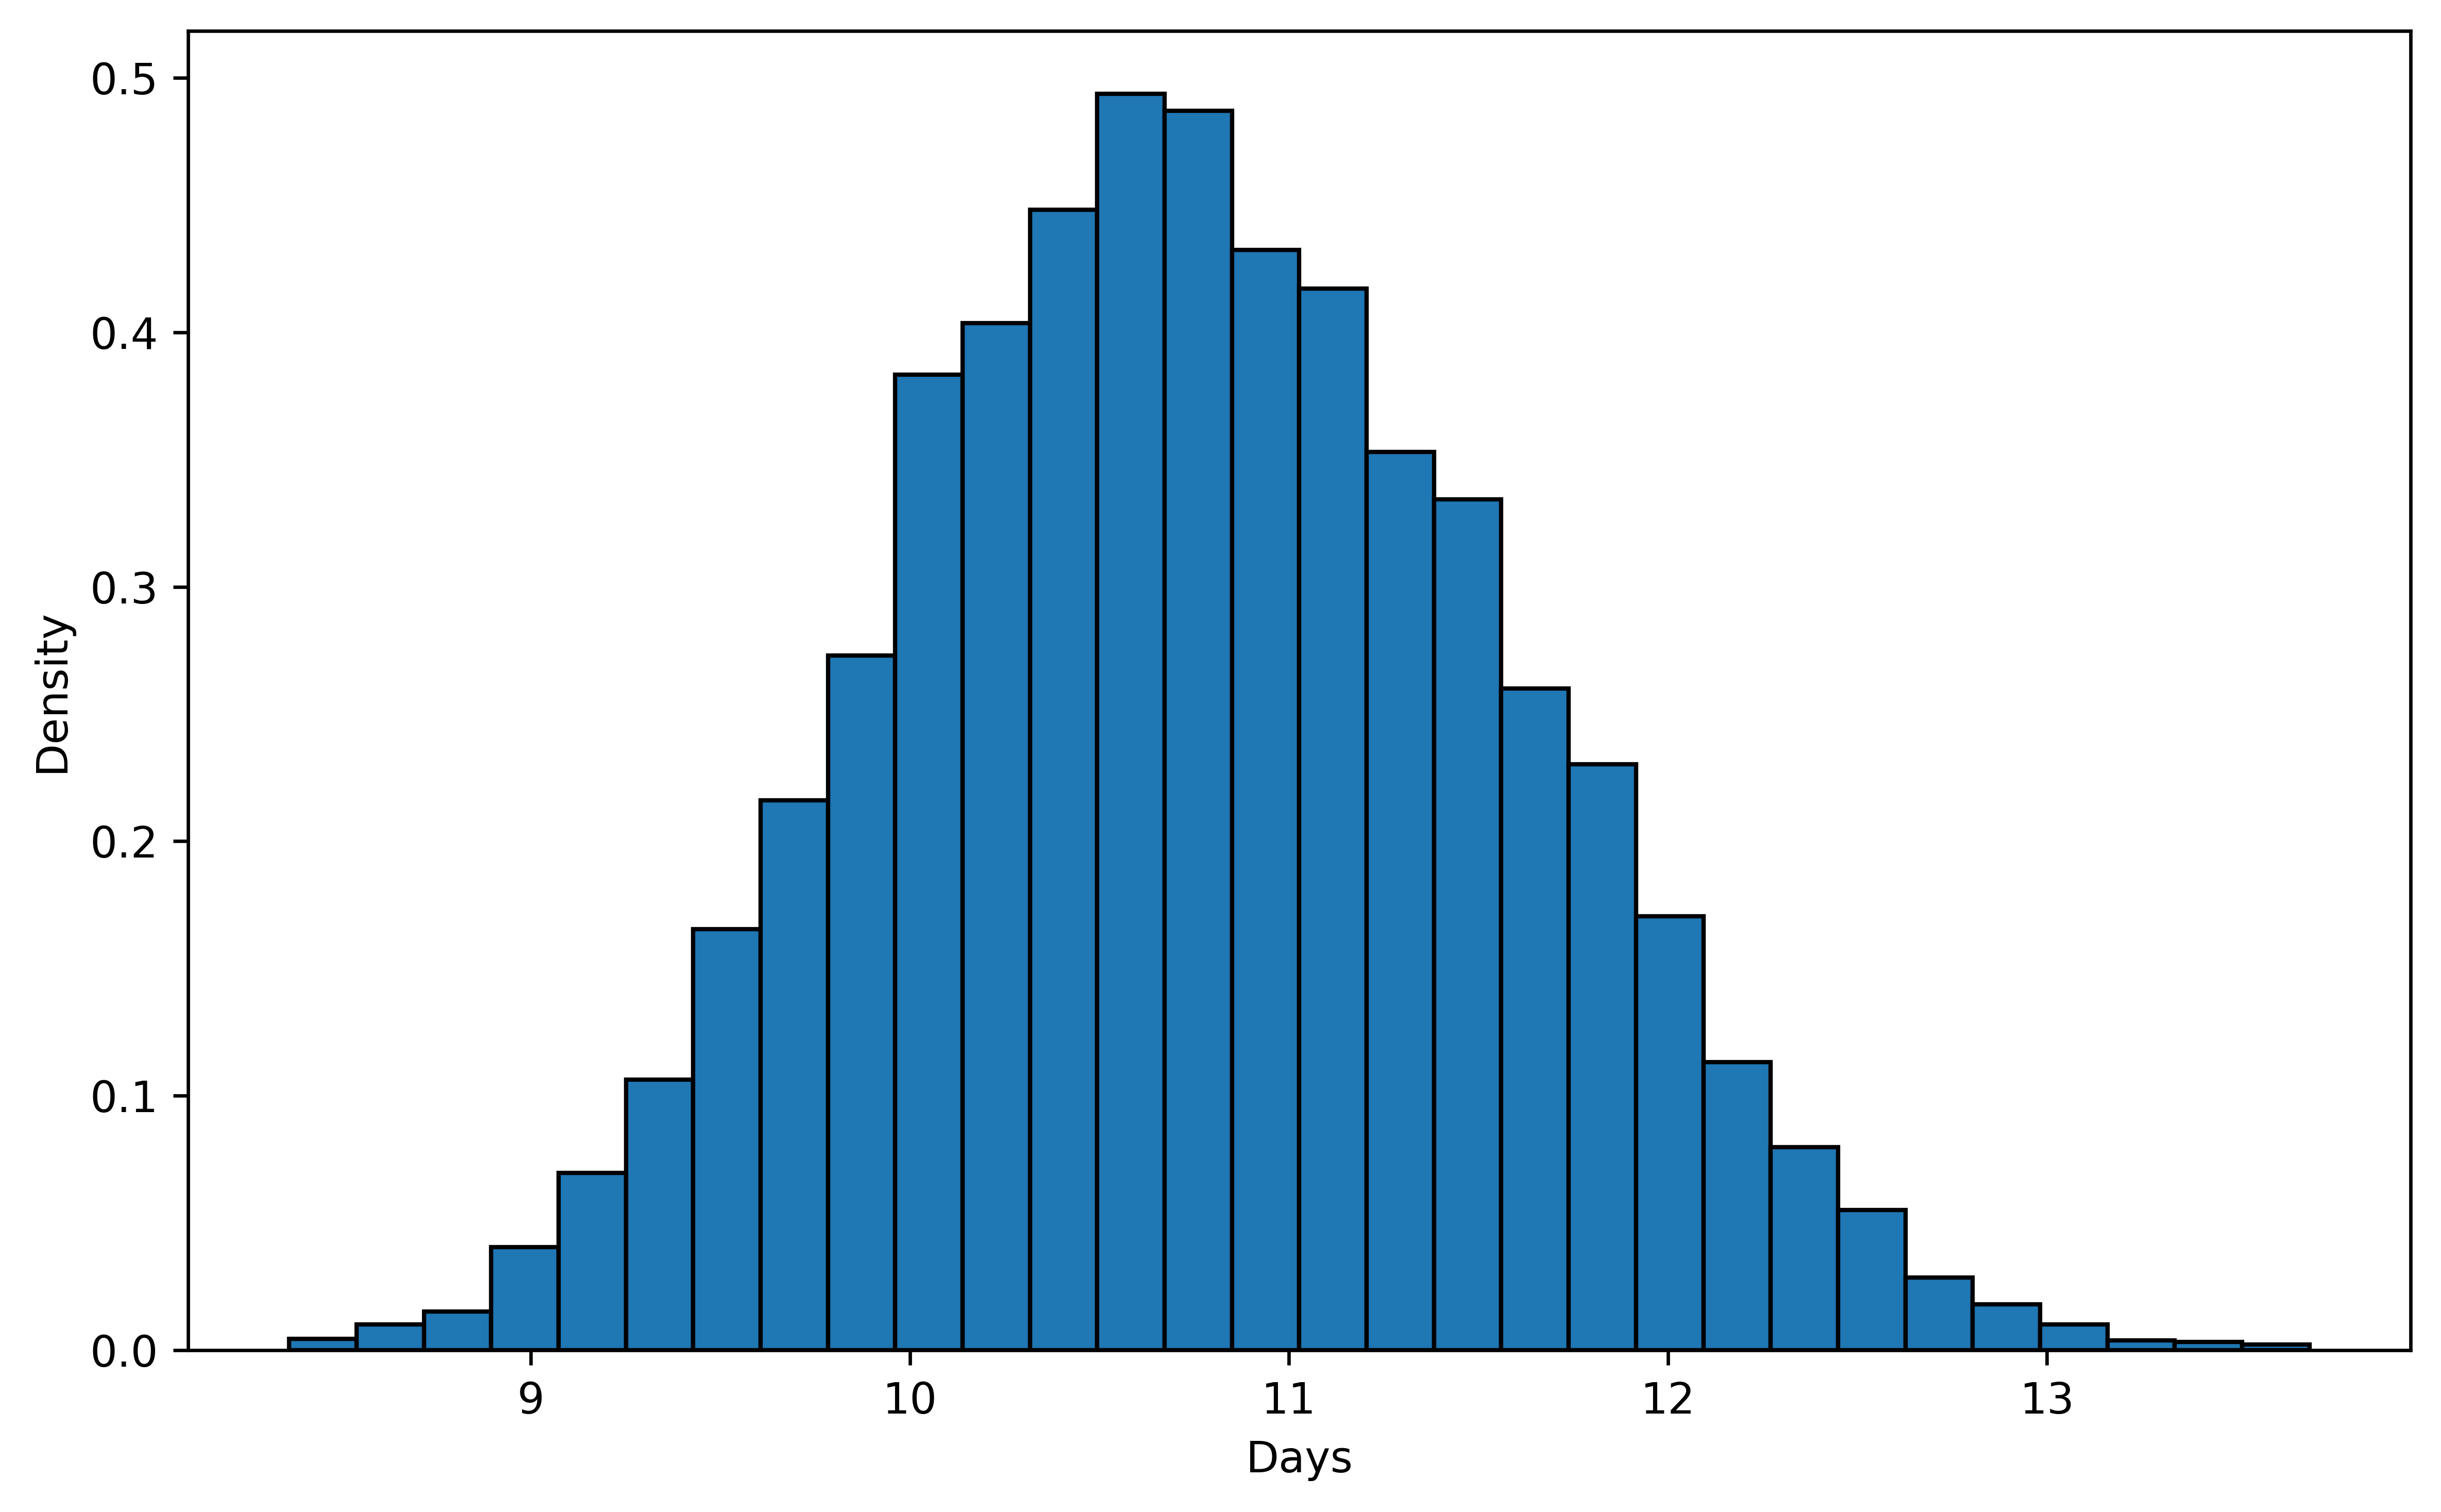
\includegraphics[width=1\linewidth]{images/makespan_distribution.png}
    \caption{Makespan distribution}
    \label{fig:makespan_scenarios}
\end{figure}

\subsubsection{Risk analysis}
%Mostra que ele faz uma análise de risco em função de um alpha declarado
%Dados os caminhos críticos calculados é possível fazer uma análise de risco, onde é possível definir com um certo indice de confiança, qual será o tempo máximo de duração do planejamento, e caso venha a ultrapassar esse valor, qual será o valor médio que pode durar. Para o calcúlo basta inserir o indice de confiança no input, conforme a figura \ref{fig:risk_analysis}. Nessa figura é mostrado que para um índice de confiança de 0.95, que o Var é de cerca de 12.20 dias e o CVar é de 12.53 dias. Para o caso onde o índice de confiança é de 0.8 o Var cai para 11.48 dias e o Cvar para 11.95, e caso o índice seja 0.5 o Var será 10.75 dias e o Cvar 11.43 dias. Isso mostra que esse tipo de problema, quanto menor o índice de confiança esperado, menor será o valor

Given the simulated critical paths, we can perform a thorough risk analysis. For instance, we can define, with a certain confidence level, the maximum duration of the planning, and if it exceeds that value, what the average duration could be. To calculate these statistics, we simply enter the confidence level as an input in the system, as depicted in figure \ref{fig:risk_analysis}. This figure shows that, for a confidence level of 0.95, i.e., $\alpha = 5\%$ the $VaR_{5\%}$ is approximately 12.20 days and the $CVaR_{5\%}$ is 12.53 days. Therefore, the results show that, for this toy exercise, the critical path will not last more than the 12.20 days, with a 95\% confidence. There is only a 5\% probability of the project makespan exceeding the $VaR$ 12.20 days. In the scenarios that the project makespan lasts more than 12.20 days, the average of the duration of the project will be $CVaR$ of 12.53 days. 

Given that the simulated scenarios allow building a probability distribution, results for other confidence levels can also be calculated, leading to a more thorough analysis of the risk of the makespan. For example, using a confidence level of 0.8, the $CVaR_{20\%}$ drops to 11.48 days and the $CVaR_{20\%}$ to 11.95 days. and if the confidence level is 0.5, the $VaR_{50\%}$ is 10.75 days and the $CVaR_{50\%}$ 11.43 days. %This shows that for this type of problem, the lower the expected confidence level, the lower the value will be.

%\begin{figure}
%    \centering
%    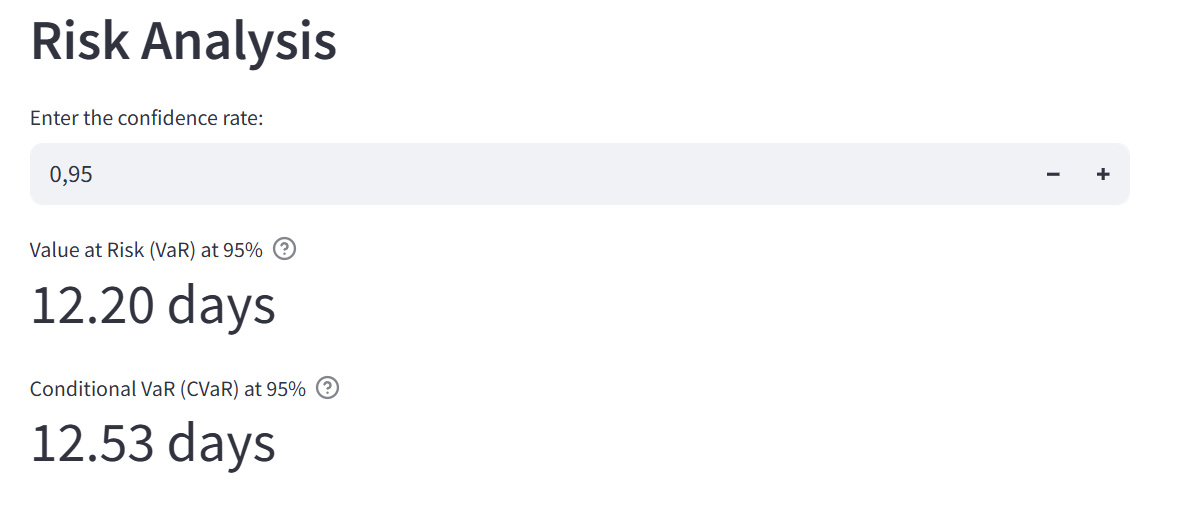
\includegraphics[width=1\linewidth]{images/risk_analysis.png}
%    %\caption{Calculo da análise de risco realizado}
%    \caption{Risk analysis}
%    \label{fig:risk_analysis}
%\end{figure}

\subsubsection{Belief updating}
%Mostra como a propação de evidência é feita no projeto

%Por fim, o sistema treina uma rede Bayesiana usando a CPT dos dados, tendo esse modelo treinado é possível fazer inferências no sistema para recalcular qual será o possível tempo total para a conclusão do projeto, na figura \ref{fig:inference} é possível ver um exemplo de inferência, onde foi informado que a atividade 1 durou extamente 2 dias, com isso, é possível ver qual será a nova previsão em dias para concluir todo o projeto na figura \ref{fig:inferece-result}.

% Finally, the system trains a Bayesian network using the CPT of the data. With this trained model, it is possible to make inferences in the system to recalculate the possible total time for the project completion. Figure \ref{fig:inference} shows an example of this inference, where it was reported that activity 1 lasted exactly 2 days. Therefore, it is possible to see the new prediction in days to complete the entire project in Figure \ref{fig:inference-result}, given the information from activity 1.


%Para demonstração da propoagração de evidências 3 cenários foram estabelecidos e verificados para a determinação da probilidade de duração da atividade final. Os cenários (a) atvidade A com 1 dia e as outros obtidas pro meios de propgarção na rede, (b) Cenários atividade A com 3 dias e atividade B com 4 dias e as outras atividades por meio da rede.


%No cenário A é possível perveber que a quando a atividade A demora 1 dia o cenário mais provável de finalização do empreendimento é de xx dias com probailidade de 0.38. 

%\textcolor{red}{Aprimorar a discussao, indicando a utilidade. In the scenario A, we can identify that, when activity A lasts 1 day, the project is more likely to be completed in XX with a 0.38 probability.}

 
Finally, the system trains a Bayesian network using the CPT derived from the data. With this trained model, it is possible to perform inferences to recalculate the total time for project completion based on real-time updates. Figure \ref{fig:inference} illustrates the interface used for this process, where an evidence was reported: activity 1 lasted exactly 2 days. Figure \ref{fig:inference}.

\begin{figure}[h]
    \centering
    \fbox{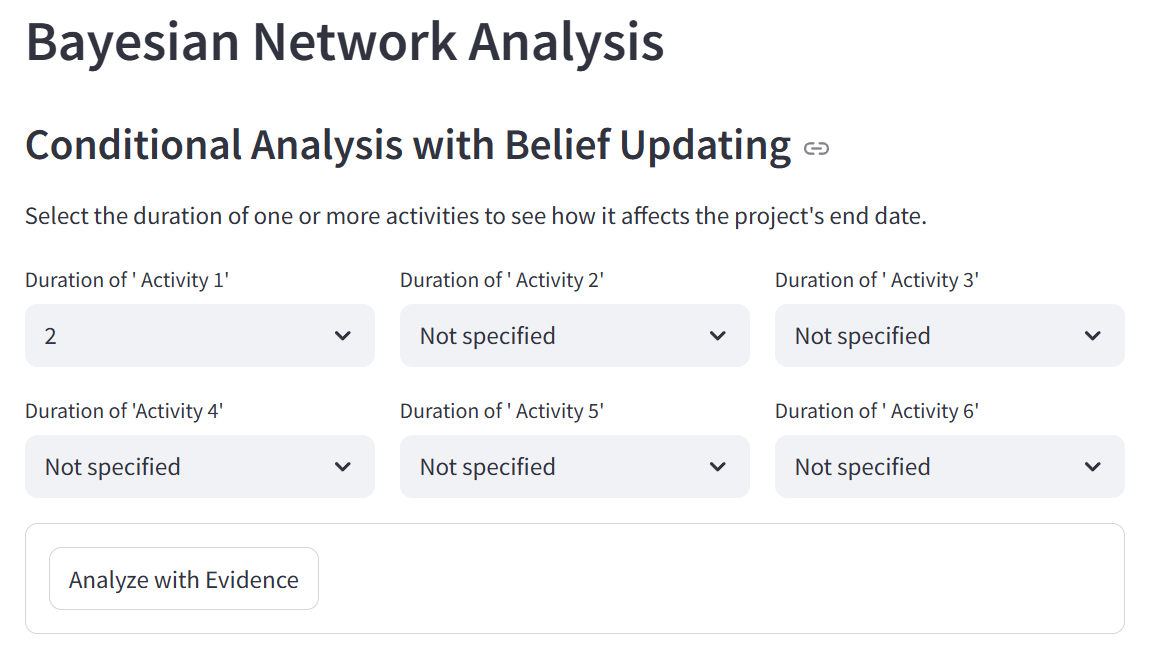
\includegraphics[width=0.8\linewidth]{images/inference.png}}
    \caption{System illustration: Interface for evidence input in the Bayesian Network, showing the selection of observed duration for Activity 1.}
    \label{fig:inference}
\end{figure}

Consequently, the updated prediction for the project makespan is presented in Figure \ref{fig:inference-result}. For this specific inference, the statistical analysis reveals an expected project makespan (mean) of 10.77 days, with a median of 10.75 days and a standard deviation of 0.82 days. The simulated scenarios for this condition range from a minimum of 8 days to a maximum of 14 days, with the most probable completion time occurring at 10 days, presenting a probability of 0.38.

To demonstrate the propagation of evidence, two additional scenarios were established to determine the probability of the final project duration: (a) activity A lasting 1 day, and (b) activity A lasting 3 days combined with activity B lasting 4 days.

\begin{figure}[h]
    \centering
    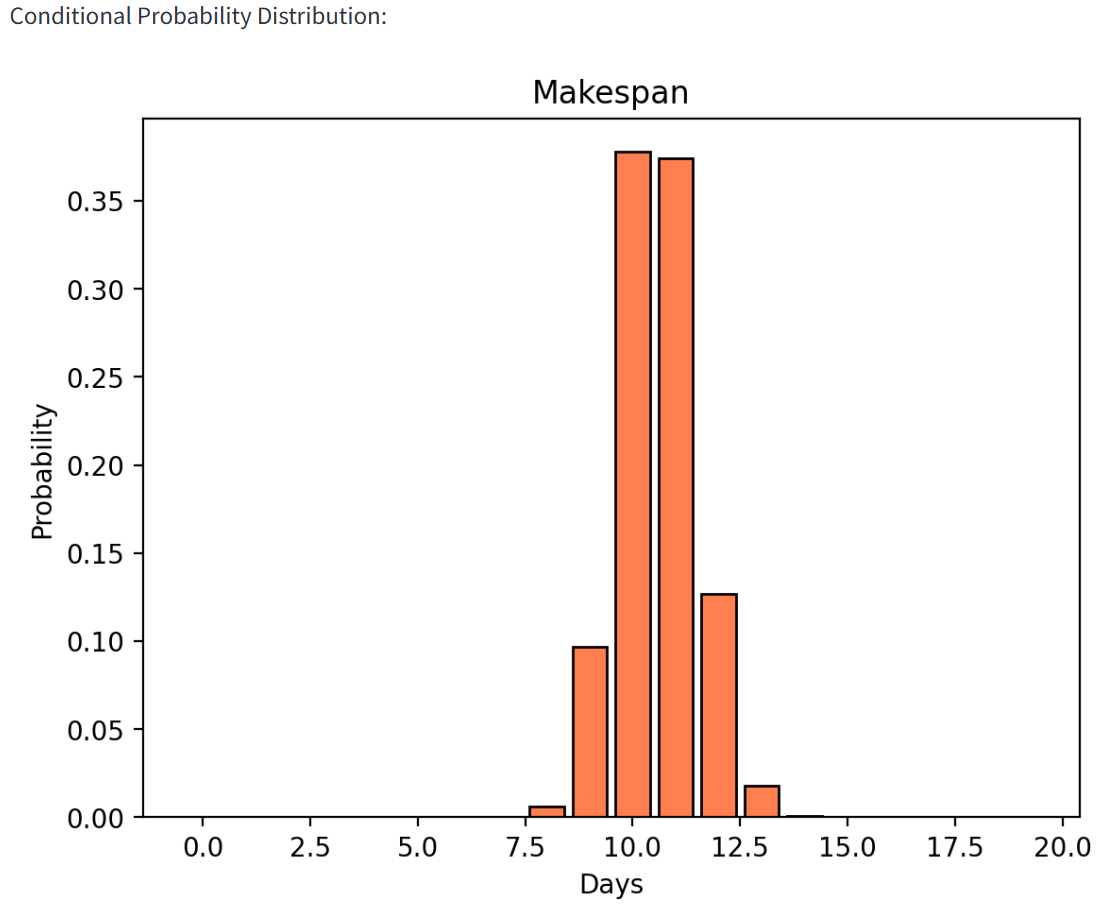
\includegraphics[width=0.8\linewidth]{images/inference_result.png}
    \caption{Probability distribution of the project makespan (Conditional PMF) after evidence propagation for different scenarios.}
    \label{fig:inference-result}
\end{figure}

The results demonstrate the model's utility for dynamic risk management. In Scenario A, when activity A lasts 1 day, the project is most likely to be completed in 9 days ($p=0.38$), within a window of 7 to 13 days. In contrast, Scenario B (Activity A=3 and B=4) shifts the distribution towards a longer duration, where the most probable outcome is 11 days ($p=0.42$), with a tighter range starting at 10 days and reaching a maximum of 14 days. This comparative analysis highlights how the Bayesian approach allows managers to quantify the impact of early task variations on the final deadline, providing a probabilistic confidence interval that is more robust than traditional deterministic methods.
\section{Results}\label{sec:res}The study presents a Digital Twin framework for risk assessment in construction scheduling, combining traditional PERT/CPM techniques with Monte Carlo simulation and Bayesian Networks. The framework uses probabilistic analysis based on financial risk management metrics, such as Value-at-Risk (VaR) and Conditional Value-at-Risk (CVaR), to evaluate uncertainty in project duration.

The model was implemented in a Python-based client-server system with a Streamlit interface, allowing updates of project duration estimates and providing a more adaptive approach for construction planning under uncertainty.

The paper contributes to the literature by combining concepts from construction scheduling, probabilistic modeling, and Digital Twin systems. The Bayesian Network structure allows updating predictions when new evidence is available. From a practical perspective, the framework can support project managers in risk assessment and monitoring activities.

However, the study has relevant limitations. The framework was tested using a simplified toy problem, which may not represent the complexity of real construction projects. In addition, activity durations were modeled using triangular distributions, which may simplify real uncertainties and dependencies. Furthermore, the proposed framework operates more as a digital shadow than a fully integrated digital twin.

Future studies could apply the framework to real construction projects, integrate real-time sensing technologies, and explore more advanced inference and automation mechanisms.

\section{Concluding remarks}\label{sec:conc}This paper presented a Digital Twin framework for risk assessment in construction scheduling, integrating traditional PERT/CPM methods with probabilistic approaches like Monte Carlo simulation and Bayesian Networks. By adapting financial risk metrics—Value-at-Risk (VaR) and Conditional Value-at-Risk ($CVaR$)—the proposed model offers a more granular and realistic perspective on project delays than traditional deterministic approaches.

\subsection{Key Contributions}
\begin{itemize}
    \item \textbf{Adoption of the Digital Shadow Paradigm:} The bibliographic review and field investigation revealed that the deployment of large-scale sensing infrastructure is rarely feasible in civil engineering projects, particularly during early planning stages. The adoption of a digital shadow approach, supported by standardized spreadsheet-based data ingestion, proved to be a fast and effective alternative for incorporating project data of varied nature into a unified probabilistic framework. This positioning makes the tool especially valuable for scenario analysis in the early phases of a project, when sensor-based monitoring is not yet justified or available.
    \item \textbf{Dynamic Decision-Making:} Unlike static deterministic plans, the framework enables project managers to update completion forecasts as activities are concluded. By propagating observed evidence through the Bayesian network, the model automatically recalculates the probability distributions of all dependent activities, supporting evidence-based replanning throughout the project lifecycle.
    \item \textbf{Risk Quantification:} The integration of Value-at-Risk (VaR) and Conditional Value-at-Risk (CVaR) provides quantile-based risk metrics that translate probabilistic schedule outputs into actionable thresholds (e.g., a 95\% probability that project duration will not exceed a given value, and the expected duration in the worst 5\% of scenarios). These metrics are essential for managing stakeholder expectations, contractual deadlines, and financial penalties.
    \item \textbf{Practical Implementation:} Developed in Python with a Streamlit-based web interface, the tool demonstrates how complex probabilistic methods, often confined to academic environments, can be translated into an intuitive experience accessible to engineering practitioners. The standardized data ingestion pipeline also favors reproducibility and facilitates the application of the framework to projects of different scales and natures.
\end{itemize}

\subsection{Limitations and Future Work}
While the framework successfully demonstrated its utility through a toy problem, some limitations remain to be addressed in future research:
\begin{itemize}
    \item \textbf{Activity Interdependence:} The current model assumes relative independence between activity durations. In real-world scenarios, external factors such as adverse weather conditions can cause correlated delays across multiple tasks. Future studies should explore modeling these common-cause failures within the Bayesian Network structure.
    \item \textbf{Data Range Constraints:} Inferences are currently restricted to the duration ranges (minimum and maximum) defined in the original dataset. Expanding the model to handle "out-of-bounds" observations would increase its resilience to extreme, unforeseen events.
    \item \textbf{Automation Maturity:} Moving from a Digital Shadow (unidirectional data flow) toward a fully integrated Digital Twin—where real-time sensor data updates the schedule automatically in both directions—remains a promising frontier for this research.
\end{itemize}

In conclusion, this framework provides construction managers with a robust, data-driven tool to navigate the inherent uncertainties of complex projects, shifting the paradigm from reactive scheduling to proactive, probabilistic risk management.


\section{Introduction2}

Your introduction goes here! Simply start writing your document and use the Recompile button to view the updated PDF preview. Examples of commonly used commands and features are listed below to help you get started.
\lipsum[2]

Once familiar with the editor, you can find various project settings in the Overleaf menu, accessed via the button at the top left of the editor. To view tutorials, user guides, and further documentation, please visit our \href{https://www.overleaf.com/learn}{help library}, or head to our plans page to \href{https://www.overleaf.com/user/subscription/plans}{choose your plan}. 

This is an example of a new paragraph with a numbered footnote\footnote{\url{https://data.gov.uk/}} and a second footnote marker.\footnote{Example of footnote text.}


%--- Section ---%
\section{Example of first level head - section head}\label{sec2}

\lipsum[4]

\lipsum[4]


\subsection{How to create sections and subsections}
Simply use the section and subsection commands, as in this example document! With Overleaf, all the formatting and numbering is handled automatically according to the template you've chosen. If you're using the Visual Editor, you can also create new sections and subsections via the buttons in the editor toolbar.

\subsection{This is an example of second level head - subsection head}\label{subsec1}
\lipsum[5]

\subsubsection{This is an example of third level head - subsubsection head}\label{subsubsec1}
\lipsum[6]

\subsubsubsection{This is an example of fourth level head - paragraph head}
\lipsum[7]


%--- Section ---%
\section{Example of first level head}\label{sec3}

\subsection{This is an example of second level head - subsection head}\label{subsec2}

\subsubsection{This is an example of third level head - subsubsection head}\label{subsubsec2}
\lipsum[8]

\subsubsubsection{This is an example of fourth level head - paragraph head}
\lipsum[9]


%--- Section ---%
\section{How to include equations}\label{sec4}

Equations in \LaTeX{} can either be inline or set as display equations. For
inline equations use the \verb+$...$+ commands. Eg: the equation
$H\psi = E \psi$ is written via the command \verb+$H \psi = E \psi$+.

For display equations (with auto generated equation numbers)
one can use the equation or eqnarray environments:
\begin{equation}
\|\tilde{X}(k)\|^2 \leq\frac{\sum\limits_{i=1}^{p}\left\|\tilde{Y}_i(k)\right\|^2+\sum\limits_{j=1}^{q}\left\|\tilde{Z}_j(k)\right\|^2 }{p+q},
\label{eq1}
\end{equation}
where
\begin{align}
D_\mu &=  \partial_\mu - ig \frac{\lambda^a}{2} A^a_\mu \nonumber \\
F^a_{\mu\nu} &= \partial_\mu A^a_\nu - \partial_\nu A^a_\mu + g f^{abc} A^b_\mu A^a_\nu
\label{eq2}
\end{align}
Notice the use of \verb+\nonumber+ in the align environment at the end
of each line, except the last, so as not to produce equation numbers on
lines where no equation numbers are required. The \verb+\label{}+ command
should only be used at the last line of an align environment where
\verb+\nonumber+ is not used.
\begin{equation}
Y_\infty = \left( \frac{m}{\textrm{GeV}} \right)^{-3}
    \left[ 1 + \frac{3 \ln(m/\textrm{GeV})}{15}
    + \frac{\ln(c_2/5)}{15} \right]
\label{eq3}
\end{equation}
The class file also supports the use of \verb+\mathbb{}+, \verb+\mathscr{}+ and
\verb+\mathcal{}+ commands. As such \verb+\mathbb{R}+, \verb+\mathscr{R}+
and \verb+\mathcal{R}+ produces $\mathbb{R}$, $\mathscr{R}$ and $\mathcal{R}$
respectively 
%(refer Subsubsection~\ref{subsubsec3}).

Equations must be provided as editable text, either in a Word or LaTeX source file. They should be numbered consecutively through the manuscript as shown in Equations \ref{eq1}, \ref{eq2} and \ref{eq3}. In APA style, when discussing numbered equations in the text, write out the word “Equation” and give the number. For example, you would write “see Equation \ref{eq1}.”
Use no punctuation after the equation if it appears at the end of a sentence; however, it is permissible (and may even be necessary) to place some form of punctuation after it (a comma or semi-colon, for example) if it appears in the middle of the sentence and is followed by text. In any case, maintain the coherence of all sentences with equations in them.


%--- Section ---%
\section{How to include tables}\label{sec5}

Use the table and tabular environments for basic tables --- see Tables~\ref{tab1} and \ref{tab2}, for example. Table \ref{tab1} is an sample figure including table footnotes. For more information, please see this help article on \href{https://www.overleaf.com/learn/latex/tables}{tables}. 

\begin{table}[!ht]
\caption{Sample table with footnotes\label{tab1}}
\begin{threeparttable}
\begin{tabular*}{\columnwidth}{@{\extracolsep\fill}llll@{\extracolsep\fill}}
\toprule
column 1 & column 2 & column 3 & column 4\\
\midrule
row 1 & data 1 & data 2 & data 3 \\
row 2 & data 4 & data 5\tnote{1} & data 6 \\
row 3 & data 7 & data 8 & data 9\tnote{2} \\
\bottomrule
\end{tabular*}
\begin{tablenotes}
\item Source: This is an example of table footnote. This is an example of table footnote. This is an example of table footnote. This is an example of table footnote. This is an example of table footnote.
\item[1] Example of a first table footnote.
\item[2] Example of a second table footnote.
\end{tablenotes}
\end{threeparttable}
\end{table}

\begin{table*}[!ht]
\caption{Example of a lengthy table which is set to full textwidth.\label{tab2}}
\tabcolsep=0pt
\begin{threeparttable}
\begin{tabular*}{\textwidth}{@{\extracolsep{\fill}}lcccccc@{\extracolsep{\fill}}}
\toprule
& \multicolumn{3}{c}{Element 1\tnote{1}} & \multicolumn{3}{c}{Element 2\tnote{2}} \\
\cmidrule(lr){2-4}\cmidrule(lr){5-7}
Project & Energy & $\sigma_{\mathrm{calc}}$ & $\sigma_{\mathrm{expt}}$ & Energy & $\sigma_{\mathrm{calc}}$ & $\sigma_{\mathrm{expt}}$ \\
\midrule
Element 3 & 990 A & 1168 & $1547\pm12$ & 780 A & 1166 & $1239\pm100$ \\
Element 4 & 500 A & 961 & $922\pm10$ & 900 A & 1268 & $1092\pm40$ \\
\bottomrule
\end{tabular*}
\begin{tablenotes}
\item Note: This is an example of table footnote this is an example of table footnote this is an example of table footnote this is an example of~table footnote this is an example of table footnote.
\item[1] Example of a first table footnote.
\item[2] Example of a second table footnote.
\end{tablenotes}
\end{threeparttable}
\end{table*}


%--- Section ---%
\section{How to include figures}\label{sec6}

\subsection{Figures}

Figures must be inserted directly into the main text of the manuscript and should not be placed collectively at the end. All figures must be cited in the main text in numerical order, and each figure should be placed immediately after the paragraph in which it is first mentioned.

All figures must be presented in a size and format that ensure clear readability. Each figure must be accompanied by an appropriate caption or legend. Figures should be numbered consecutively throughout the manuscript using Arabic numerals (for example, Figure 1, Figure 2, and Figure 3). For figures appearing in an appendix, the numbering should be prefixed with the appendix letter (for example, Figure A1 and Figure B1).

Authors are strongly encouraged to use two-dimensional (2D) graphics rather than three-dimensional (3D) graphics unless a 3D representation is essential, as 2D graphics are generally clearer, more accurate, and easier to interpret. Border lines around figures should be removed. Authors should also avoid the use of white text and background colors in figures, as these may reduce legibility.

When referring to figures in the manuscript text and in figure captions, authors must use the full term “Figure” rather than the abbreviation “Fig.”

Note that your figure will automatically be placed in the most appropriate place for it, given the surrounding text and taking into account other figures or tables that may be close by. You can find out more about adding images to your documents in this help article on \href{https://www.overleaf.com/learn/how-to/Including_images_on_Overleaf}{including images on Overleaf}.



\begin{figure}[!ht]
\centering
\includegraphics[width=0.5\linewidth]{cat_momo_1.png}
\caption{\label{fig:cat1}This cat picture is located at the 'figures' folder.}
\end{figure}


If a figure consists of multiple subfigures as shown in Figure 2, each subfigure should be identified by a capital letter, such as (A), (B), (C), and so forth, centered below the corresponding subfigure. Authors should follow the style illustrated in Figure 2 of the manuscript template. Subfigure labels must not be embedded within the image itself.

When citing a figure that contains multiple subfigures in the main text, authors should use the format Figure 2A, Figure 2B, and so on. In the figure caption, the corresponding descriptions should be given using the format (A), (B), (C), etc.

When multiple images are combined into a single figure using a grid arrangement, authors should ensure that the layout does not compromise visibility. In particular, placing too many images in a single horizontal row may reduce the size of each image and make textual or graphical details difficult to read. Where necessary, authors should reduce the number of images arranged horizontally. For example, if a 2 × 4 layout results in images that are too small, a 4 × 2 layout may provide better visibility.


\begin{figure}[!ht]
    \centering
    \begin{subfigure}{0.45\textwidth}
        \includegraphics[width=\linewidth]{fig_a.png}
        \caption{}
    \end{subfigure}
    \hfill
    \begin{subfigure}{0.45\textwidth}
        \includegraphics[width=\linewidth]{fig_b.png}
        \caption{}
    \end{subfigure}
    \vskip\baselineskip
    \begin{subfigure}{0.45\textwidth}
        \includegraphics[width=\linewidth]{fig_c.png}
        \caption{}
    \end{subfigure}
    \hfill
    \begin{subfigure}{0.45\textwidth}
        \includegraphics[width=\linewidth]{fig_a.png} % 첫 번째 그림 다시 사용
        \caption{}
    \end{subfigure}
    \caption{Overall caption for the four figures. (A) Caption for figure A. (B) Caption for figure B. (C) Caption for figure C. (D) Caption for figure D.}
    \label{fig:multi_figs}
\end{figure}

\subsection{Alt text}

Incorporating alt text (alternative text) when submitting your paper helps to foster inclusivity and accessibility. Well-written alt text enables readers with visual impairments, including those using screen readers, to understand the content and context of your figures. The purpose of alt text is to provide concise, informative descriptions of the essential information conveyed by each figure so that all readers have equitable access to the same information and can engage with the visual elements integral to scholarly content. Including alt text demonstrates a commitment to accessibility and can enhance the overall impact and reach of your work. Although some journals include alt text below each figure caption, as shown in Figure \ref{fig:alt_text}, for administrative convenience we ask authors to submit a separate MS Word file containing a list of all alt texts once the manuscript has been accepted.
Please note the following points regarding alt text:
\begin{itemize}
\item Alt text applies to all images, figures, illustrations, and photographs.
\item Alt text is primarily accessed via assistive technologies (e.g., screen readers) and may not appear in the typeset article.
\item Once the manuscript has been accepted, please submit alt text in a separate MS Word file.
\item \href{https://static.primary.prod.gcms.the-infra.com/static/site/journals/document/alt-text-figure-accessibility.pdf?node=1329505d4d63d87a12ed}{Detailed guidance on how to draft and submit alt text.}
\end{itemize}


\begin{figure}[!ht]
\centering
\includegraphics[width=0.7\linewidth]{alt_text_example.png}
\caption{\label{fig:alt_text}Completely confined, partially deconfined, and completely deconfined phases correspond to uniform, nonuniform but jointed, and disjointed distributions of Polyakov line phases, respectively.\\
\textbf{Alt Text:} Graphical representation of three phases—completely confined, partially deconfined, and completely deconfined—depicting Polyakov line phases with corresponding transition profiles.
}
\end{figure}

%--- Section ---%
\section{How to include algorithms, program codes, and listings}\label{sec8}
Packages \verb+algorithm+, \verb+algorithmicx+, and \verb+algpseudocode+ are used for setting algorithms in latex.
For this, one has to use the below format:

\begin{verbatim}
\begin{algorithm}
\caption{<alg-caption>}\label{<alg-label>}
\begin{algorithmic}[1]
. . .
\end{algorithmic}
\end{algorithm}
\end{verbatim}

You may need to refer to the above-listed package documentation for more details before setting an \verb+algorithm+ environment.
To set program codes, one has to use the \verb+program+ package. We need to use the \verb+\begin{program}+ \verb+...+
\verb+\end{program}+ environment to set program codes.

\begin{algorithm}[!ht]
\caption{Calculate $y = x^n$}\label{algo1}
\begin{algorithmic}[1]
\Require $n \geq 0 \vee x \neq 0$
\Ensure $y = x^n$
\State $y \Leftarrow 1$
\If{$n < 0$}
        \State $X \Leftarrow 1 / x$
        \State $N \Leftarrow -n$
\Else
        \State $X \Leftarrow x$
        \State $N \Leftarrow n$
\EndIf
\While{$N \neq 0$}
        \If{$N$ is even}
            \State $X \Leftarrow X \times X$
            \State $N \Leftarrow N / 2$
        \Else[$N$ is odd]
            \State $y \Leftarrow y \times X$
            \State $N \Leftarrow N - 1$
        \EndIf
\EndWhile
\end{algorithmic}
\end{algorithm}

Similarly, for \verb+listings+, one has to use the \verb+listings+ package. To set environments similar to the \verb+verbatim+ environment, the \verb+\begin{lstlisting}+ \verb+... + \verb+\end{lstlisting}+ environment is used . Refer to the \verb+lstlisting+ package documentation for more details on this.

\begin{minipage}{\hsize}%
\lstset{language=Pascal}% Set your language (you can change the language for each code-block optionally)
\begin{lstlisting}[frame=single,framexleftmargin=-1pt,framexrightmargin=-17pt,framesep=12pt,linewidth=0.95\textwidth]
for i:=maxint to 0 do
begin
{ do nothing }
end;
Write('Case insensitive ');
Write('Pascal keywords.');
\end{lstlisting}
\end{minipage}


%--- Section ---%
\section{How to include lists}\label{sec7}

List in \LaTeX{} can be of three types: numbered, bulleted, and unnumbered. The ``enumerate'' environment produces a numbered list, the 
``itemize'' environment produces a bulleted list, and the ``unlist''
environment produces an unnumbered list.
In each environment, a new entry is added via the \verb+\item+ command.

\begin{enumerate}[label=\arabic*.]
\item This is the 1st item
\item Enumerate creates numbered lists, itemize creates bulleted lists, and unnumerate creates unnumbered lists.

\begin{enumerate}[label=\alph*.]
\item Second level numbered list. Enumerate creates numbered lists, itemize creates bulleted lists, and description creates unnumbered lists.
\item Second level numbered list. Enumerate creates numbered lists, itemize creates bulleted lists, and description creates unnumbered lists.

\begin{enumerate}[label=(\roman*)]
\item Third level numbered list. Enumerate creates numbered lists, itemize creates bulleted lists, and description creates unnumbered lists.
\item Third level numbered list. Enumerate creates numbered lists.
\end{enumerate}

\item Second level numbered list. Enumerate creates numbered lists, itemize creates bulleted lists, and description creates unnumbered lists.
\end{enumerate}

\item Numbered lists continue.
\end{enumerate}
Lists in \LaTeX{} can be of three types: enumerate, itemize, and description.
In each environment, a new entry is added via the \verb+\item+ command.

\begin{itemize}
\item First level bulleted list. This is the 1st item
\item First level bulleted list. Itemize creates bulleted lists, and description creates unnumbered lists.

\begin{itemize}
\item Second level dashed list. Itemize creates bulleted lists, and description creates unnumbered lists.
\item Second level dashed list. Itemize creates bulleted lists, and description creates unnumbered lists.
\end{itemize}

\item First level bulleted list. Bullet lists continue.
\end{itemize}

\noindent
Example of unnumbered list items:

\begin{unlist}
\item Sample unnumberd list text. Sample unnumberd list text. Sample unnumberd list text. Sample unnumberd list text. Sample unnumberd list text.

\item Sample unnumberd list text. Sample unnumberd list text. Sample unnumberd list text.

\item Sample unnumberd list text. Sample unnumberd list text. Sample unnumberd list text. Sample unnumberd list text. 
\end{unlist}


%--- Section ---%
\section{How to add citations and a references list}

You can simply upload a \verb|.bib| file containing your BibTeX entries, created with a tool such as JabRef. You can then cite entries from it, like this: \textcite{greenwade93}. Just remember to specify a bibliography style, as well as the filename of the \verb|.bib|. You can find a \href{https://www.overleaf.com/help/97-how-to-include-a-bibliography-using-bibtex}{video tutorial here} to learn more about BibTeX.

Here is an example citation when you want an author name like \textcite{collins2011a} to appear in the text. And here's how to do a parenthetic citation, when you want to mention a reference at the end of a sentence or part of a sentence \parencite{collins2013}. It is possible to cite multiple references at the same time \parencite{collins2011b,collins2016,lunn2007a,lunn2007b,ross2006,shannon1948}.

If you have an \href{https://www.overleaf.com/user/subscription/plans}{upgraded account}, you can also import your Mendeley or Zotero library directly as a \verb|.bib| file, via the upload menu in the file-tree.

\subsection{Citation in text}
Please ensure that every reference cited in the text is also present in the reference list (and vice versa). Citations in the text should follow the referencing style used by the American Psychological Association. You are referred to the Publication Manual of the American Psychological Association (APA), Seventh Edition, ISBN 978-1-4338-3215-4, copies of which may be ordered online. References in the Abstract should be avoided, but if essential, then cite the author(s) and year(s). Unpublished results and personal communications are not recommended in the reference list but may be mentioned in the text. If these references are included in the reference list, they should follow the standard reference style of the journal and should include a substitution of the publication date with either ‘Unpublished results’ or ‘Personal communication’. The citation of a reference as ‘in press’ implies that the item has been accepted for publication. 

An APA in-text citation includes only three items: the last name(s) of the author(s), the year the source was published, and sometimes the page or location of the information. More than one reference from the same author(s) in the same year must be identified by the letters ‘a’, ‘b’, ‘c’, etc., placed after the year of publication. The following paragraph shows examples of APA style of citations.

Here is an example citation when you want an author name like \textcite{collins2011a} to appear in the text. And here's how to do a parenthetic citation when you want to mention a reference at the end of a sentence or part of a sentence \parencite{collins2013}. It is possible to cite multiple references at the same time \parencite{collins2011b,collins2016,lunn2007a,lunn2007b,ross2006,shannon1948}.

The followings are examples of \verb+\textcite{...}+: \textcite{rahman2019centroidb}, \textcite{krizhevsky2012imagenet, horvath2018dna}, and \textcite{lecun2015deep, zhang2018fine, ravi2016deep}. Another example of \verb+\parencite{...}+: \parencite{bahdanau2014neural,imboden2018cardiorespiratory,motiian2017unified,murphy2012machine,ji20123d}.

\subsection{References}
The Reference Section, also called the Reference List or Cited Works List, is a list of the full-text details of the in-text citations that have been used in the main text. It includes information such as the name of the author(s), the year the source was published, the full title of the source, and the URL or page range. The Reference Section allows the reader to find the text easily and can be considered as the long-hand format of the in-text citation. It is found at the end of the piece of writing. The works in a reference section should be arranged first alphabetically and then further sorted chronologically if necessary.

\subsubsection{Web references}
As a minimum, the full URL and the date when the reference was last accessed should be given. Any further information, if known (DOI, author names, dates, reference to a source publication, etc.), should also be given. Web references can be listed separately (e.g., after the reference list) under a different heading if desired or can be included in the reference list. With standard numerical .bst files, only numerical citations are possible. With an author-year .bst file, both numerical and author-year citations are possible. 

\subsubsection{Examples of reference style}
You can find information about the examples of APA-style references to various sources at the following site:\\
\url{https://apastyle.apa.org/style-grammar-guidelines/references/examples}.


%--- Section ---%
\section{Conclusions}
Some conclusions here.

%-------------------------------------------
% Acknowledgement Sections
%-------------------------------------------

%--- Mandatory Section ---%
\section*{Conflicts of interest} 
The authors declare that they have no known competing financial interests or personal relationships that could have appeared to influence the work reported in this paper.

%--- Mandatory Section ---%
\section*{Author contributions}

\noindent\textbf{Nilson J. Leão Júnior}: Methodology, Software, Writing – original draft, and review. \textbf{Wanderlei M. Pereira Junior}: Conceptualization, Benchmarks, Supervision, Validation, Writing, and review. \textbf{Henrique O. Caetaneo}: Bayesian networks, Investigation, and Validation. \textbf{Marcos Napoleão}: Supervision, Validation, Writing, and review. \textbf{Marcos Luiz Henrique}: Graph, Validation, and Writing. \textbf{Hebert Kimura}: Risk analysis, Writing, and review. \textbf{Carlos Maciel}: Editing, Writing, and review.

%--- Section ---%
\section*{Funding}
Cite all funding for your research, providing the grant number and the funder name. An example statement is as follows: This work is supported in part by funds from the National Science Foundation (NSF: \# 1636933 and \# 1920920). 

If the funder is listed in the Crossref funder registry (\url{https://www.crossref.org/services/funder-registry/}), the funder name should appear exactly as it does in that database. Where grants were received by specific members of the author group, they should be identified by initials. 

More information on funding agency requirements is available at  \url{https://academic.oup.com/pages/open-research/open-access/complying-with-funder-policies}.

%--- Section ---%
\section*{Data availability}
The data availability statement should provide information on where and under what conditions the data directly supporting the publication can be accessed. Sample data availability statements are available at the following site: \url{https://academic.oup.com/pages/open-research/research-data#Data%20Availability%20Statements}.

%--- Section ---%
\section*{Acknowledgments}
The authors thank those people or institutions that have helped you in the preparation of the manuscript. 


%-------------------------------------------
% References
%-------------------------------------------

% Print bibliography
\printbibliography




%-------------------------------------------
% Appendix
%-------------------------------------------
% Activate the appendix in the doc
% from here on sections are numerated with capital letters 
%\appendix

% Change equation numbering format to be sequential within sections in the appendix
\renewcommand\theequation{\Alph{section}\arabic{equation}} % Redefine equation numbering format
\counterwithin*{equation}{section} % Number equations within sections
\renewcommand\thefigure{\Alph{section}\arabic{figure}} % Redefine equation numbering format
\counterwithin*{figure}{section} % Number equations within sections
\renewcommand\thetable{\Alph{section}\arabic{table}} % Redefine equation numbering format
\counterwithin*{table}{section} % Number equations within sections



\begin{appendices}


%--- For single section ---%
%\section*{Appendix}

%--- For multiple sections ---%
% Appendix formatting
\renewcommand{\thesection}{Appendix \Alph{section}}
\renewcommand{\thesubsection}{\Alph{section}.\arabic{subsection}}

%--- Section ---%
\section{Section title of first appendix}
Appendices are used for supplementary material that is relevant to the main text but not essential for inclusion in the text itself—for example, questionnaires, interview transcripts, extended data tables, or equipment descriptions.
\begin{itemize}
\item If there is only one appendix, label it as “Appendix”; if there are multiple appendices, label them as “Appendix A,” “Appendix B,” and so on, arranging them in the order they appear in the paper. 
\item All appendices must be referenced in the main text, and only items that enhance the reader’s understanding or support your argument should be included.
\item Tables and figures in an appendix should be labeled separately (e.g., Table \ref{tab_a1}, Figure \ref{fig:cat2}).
\end{itemize}

%--- Subsection ---%
\subsection{Fist subsection title of first appendix}
As shown in Equation \ref{eq_a1}, the section number is inserted in the equation number.
\lipsum[11]

\begin{equation}
Y_\infty = \left( \frac{m}{\textrm{GeV}} \right)^{-3}
    \left[ 1 + \frac{3 \ln(m/\textrm{GeV})}{15}
    + \frac{\ln(c_2/5)}{15} \right]
\label{eq_a1}
\end{equation}

%--- Subsection ---%
\subsection{Second subsection title of first appendix}
As shown in Table \ref{tab_a1}, the section number is inserted in the table number.

\begin{table}[!ht]
\caption{Sample table with three parts and five columns\label{tab_a1}}
\begin{threeparttable}
\begin{tabular*}{\columnwidth}{@{\extracolsep\fill}lllll@{\extracolsep\fill}}
\toprule
column 1 & column 2 & column 3 & column 4 & column 5\\
\midrule
row 1 & data 0 & data 1 & data 2 & data 3 \\
row 2 & data 4 & data 5 & data 6 & data 7 \\
row 3 & data 8 & data 9 & data 10 & data 11\\
\bottomrule
\end{tabular*}
\end{threeparttable}
\end{table}

%--- Subsubsection ---%
\subsubsection {Subsubsection title of first appendix}
\lipsum[12]


%--- Section ---%
\section{Section title of second appendix}

As shown in Figure \ref{fig:cat2}, the section number is inserted in the figure number.
\lipsum[13]

% figure b1
\begin{figure}[!htbp]
\centering
\includegraphics[width=0.8\linewidth]{cat_momo_2.jpg}
\caption{\label{fig:cat2}This cat picture is located at the 'figures' folder.}
\end{figure}

\lipsum[14]

\subsection{Appendix subsection title here}
\lipsum[15]

\end{appendices}

\end{document}